
\chapter{Arches}

\section{Introduction}
%
The ARCHES component was initially designed for predicting the heat-flux from large buoyant pool fires with potential hazard hazards immersed in or near a pool fire of transportation fuel.  Since then, this component has been extended to solve many industrially relevant problems such as industrial flares, oxy-coal combustion processes, and fuel gasification.  

The ARCHES component solves the conservative, finite volume, compressible, low-mach formulation of the Navier-Stokes equation with a pressure projection that includes the effect of variable density, reaction, and heat transfer modes in the gas phase including radiation.  Given the wide range of length and time scales that are present in many combustion problems of interest, ARCHES utilizes models for bridging the molecular (micro) scales to the full, large (macro) scales.  This bridging occurs through the use of subgrid and resolved scale mixing, reaction, and turbulence models. For example, momentum turbulence closure is accomplished by using various large eddy simulation (LES) type closure models. Fast chemistry scales are modeled by preprocessing the full chemical mechanism, modeled in various idealized configurations (e.g., equilibrium or flamelets), then tracking a set of reduced parameters on the LES mesh that map the full thermochemical state-space.  In general, the chemistry is tabulated and stored in a reaction table.  Subgrid turbulence species mixing processes and included by using presumed PDF methods and using models for certain moments of the distribution (e.g., scalar variance and mixture fraction).  The turbulence-species subgrid interaction model description are termed mixing models.  The chemistry and mixing models are usually completely preprocessed together into one tabular format to give a mixing table.  

Note that the sister component, MPMARCHES, couples an MPM description of a solid object to include stationary solids with and without conjugate heat transfer. While run as a separate component, MPMARCHES is simply a wrapped version of ARCHES to include the MPM interface.  

The following gives a brief introduction to a few of the key concepts of the Arches formulation of the transport equations and physical models as well as the CFD algorithm.  Following this explanation, an overview of the ARCHES input parameters are given.  

\section{Governing Equations}
%
The essential governing equations for the Arches component, written
in finite volume form, include the mass balance, momentum balance,
mixture fraction balance, and energy balance equations. Using a bold-face
symbol to represent a vector quantity, the equations are: 
\begin{enumerate}
\item The mass balance, \begin{equation}
\int_{V}\frac{\partial\rho}{\partial t}dV+\oint_{S}\rho\mathbf{u}\cdot d\mathbf{S}=0\;,\label{eqn:mass_balance}\end{equation}
 where $\rho$ is density and $\mathbf{u}$ is the velocity vector. 
\item The momentum balance, \begin{equation}
\int_{V}\frac{\partial\rho\mathbf{u}}{\partial t}dV+\oint_{S}\rho\mathbf{uu}\cdot d\mathbf{S}=\oint_{S}\tau\cdot d\mathbf{S}-\int_{V}\nabla pdV+\int_{V}\rho\mathbf{g}dV\;,\label{eqn:mom_balance}\end{equation}
 where $\tau$ is the deviatoric stress tensor defined as $\tau_{ij}=2\mu S_{ij}-\frac{2}{3}\mu\frac{\partial u_{k}}{\partial x_{k}}\delta_{ij}$,
the second isotropic term in $\tau_{ij}$ is absorbed into the pressure
projection for the current low-Mach scheme, and $S_{ij}=\frac{1}{2}\left(\frac{\partial u_{i}}{\partial x_{j}}+\frac{\partial u_{j}}{\partial x_{i}}\right)$.
Also in Equation \ref{eqn:mom_balance}, $\mathbf{g}$ is the gravitational
body force and $p$ is pressure. 
\item The mixture fraction balance, \begin{equation}
\int_{V}\frac{\partial\rho f}{\partial t}dV+\oint_{S}\rho\mathbf{u}f\cdot d\mathbf{S}=\oint_{S}D\nabla f\cdot d\mathbf{S}\;,\label{eqn:species_balance}\end{equation}
 where $f$ is the mixture fraction and a Fick's law form of the diffusion
term assuming equal diffusivities results in a single diffusion coefficient,
$D$. 
\item The thermal energy balance, \begin{equation}
\int_{V}\frac{\partial\rho h}{\partial t}dV+\oint_{S}\rho\mathbf{u}h\cdot d\mathbf{S}=\oint_{S}k\nabla h\cdot d\mathbf{S}-\oint_{S}q\cdot d\mathbf{S}\;,\label{eqn:heat_balance}\end{equation}
 where $h$ is the sum of the chemical plus sensible enthalpy, $q$
is the radiative flux, a Fourier's law form of the conduction term
is used with a diffusion coefficient, $k$, and the pressure term
is neglected. 
\end{enumerate}
These equations are solved in an LES context, meaning filters are
applied to the equations. Here, we use Favre filtering, defined as
\[
\overline{\phi}=\frac{\overline{\rho\phi}}{\overline{\rho}},\]
 to isolate the density in the filtered equations. The filtering operations
result in the classic turbulence closure problem and thus models are
required. 

Consider a control volume, $V$, with surface area $S$.  Because the equations will be  solved on a computational grid, one can safely assume that the the control volume has $N$ faces, where unique faces are identified with their index, $k$.  The discussion is further simplified by only considering cubic volumes with length $h$.  
Given the cubic control volume, a surface-filtered field for a variable $\phi$ is defined as $\overline{\phi}^{(j)}(\mathbf{x})$, where the variable is filtered on a plane in the $x_j$ orthogonal direction.  Then, for any surface, $k$, the field is sampled at the face centered location.  For example, if $j=1$, the surface-filtered quantity is
%
\begin{equation}
\overline{\phi}^{2d, (1)}(\mathbf x) = \frac{1}{h^2} \int_{x_2 - h/2}^{x_2 + h/2}  \int_{x_3 - h/2}^{x_3 + h/2} \phi(\mathbf x') dx_2' dx_3' \; .
\end{equation} 
%
The volume average follows as
%
\begin{equation}
\overline{\phi}^{3d} (\mathbf x) = \frac{1}{h^3} \int_{x_1 - h/2}^{x_1 + h/2} \int_{x_2 - h/2}^{x_2 + h/2}  \int_{x_3 - h/2}^{x_3 + h/2} \phi(\mathbf x') dx_1' dx_2' dx_3' \; .
\end{equation}
%
The bars over the variable, $\phi$, are labeled with `2d' and `3d' superscripts to distinguish between the two filters.  Pope \cite{Pope179} identifies the proceeding definitions as using the ``anisotropic box" filter kernel where the resultant variables are simply averages over the intervals $x_j - \frac{1}{2}h < x_j' < x_j + \frac{1}{2}h$. 

For convenience in isolating density in the filtered equations, a Favre-filtered quantity is defined for an arbitrary variable, $\varphi$, as 
%
\begin{equation}\label{eqn:favre_surf}
\widetilde{\varphi}^{2d} \equiv \frac{\overline{\rho \varphi}^{2d}}{\overline{\rho}^{2d}} \; ,
\end{equation}
%
and
%
\begin{equation}\label{eqn:favre_vol}
\widetilde{\varphi}^{3d} \equiv \frac{\overline{\rho \varphi}^{3d}}{\overline{\rho}^{3d}} \;.
\end{equation}
%
Because the 2d and 3d filters are explicitly defined, this convention is slightly different than what is normally observed in the literature.  Most literature, however, derives the filtered equations from the finite difference equations rather than the finite volume equations.  Thus, using $\overline{\rho}^{2d}$ and $\overline{\rho}^{3d}$ in Equations \ref{eqn:favre_surf} and \ref{eqn:favre_vol} to stress surface and volume filtered densities are appropriate for the present discussion.

The previous definitions are applied to the integral forms of the governing equations to obtain the Favre-filtered LES equations.  Nevertheless, there are terms in the Favre-filtered equations that cannot be solved.  These include the surface filtered convection of momentum, $\widetilde{u_i u}^{2d}_j$, the surface filtered convection of mixture fraction, $\widetilde{u_j f}^{2d}$, and the surface filtered convection of enthalpy, $\widetilde{u_j h}^{2d}$.  

For the filtered velocity product, $\overline{\rho}^{2d} \; \widetilde{ u_i u}^{2d}_j$, a subgrid stress tensor is defined as, 
%
\begin{equation}\label{eqn:tau_sgs}
\tau^{sgs}_{ij} = \widetilde{u_i u}^{2d}_j - \widetilde{u}^{2d}_i \widetilde{u}^{2d}_j \; .
\end{equation}
%
Similarly, subgrid diffusion terms are defined for mixture fraction and enthalpy, 
%
\begin{eqnarray}
\mathcal{J}^{f}  = \widetilde{u_j f}^{2d} - \widetilde{u}^{2d}_j \widetilde{f}^{2d} \;, \\
\mathcal{J}^{h} = \widetilde{u_j h}^{2d} - \widetilde{u}^{2d}_j \widetilde{h}^{2d} \; .\\
\end{eqnarray}

Using these definitions, the final form of the Favre-filtered equations is
%
\begin{enumerate}
\item The filtered mass balance, 
%
\begin{equation}\label{eqn:filtered_mass_balance}
\frac{d}{d t} \left(\widetilde{\rho}^{3d} \right)   + \frac{S_k}{V} n_{kj} \left( \overline{\rho}^{2d} \; \widetilde{u}^{2d}_j \right) = 0 \; .
\end{equation}
%
\item The filtered momentum balance, 
%
\begin{equation}\label{eqn:filtered_mom_balance}
\frac{d}{d t} \left( \overline{\rho}^{3d} \; \widetilde{u}^{3d}_i \right) = \frac{S_{k}}{V} n_{kj}\left( -\overline{\rho}^{2d} \; \widetilde{u}^{2d}_i\widetilde{u}^{2d}_j + \overline{\tau}^{2d}_{ij} + \tau^{sgs}_{ij} - \overline{p}^{2d} \delta_{ij} \right) + \overline{\rho}^{3d} \; g_i  \; .
\end{equation}
%
\item The filtered mixture fraction balance,
%
\begin{equation}\label{eqn:filtered_mixfrac_balance}
\frac{d}{d t} \left( \overline{\rho}^{3d} \; \widetilde{f}^{3d} \right) = \frac{S_k}{V} n_{kj} \left( -\overline{\rho}^{2d} \; \widetilde{u}^{2d}_j \widetilde{f}^{2d} + D \nabla \overline{f}^{2d} + \mathcal{J}^{f} \right) \; .
\end{equation}
%
%
\item The filtered thermal energy balance, 
%
\begin{equation}\label{eqn:filtered_heat_balance}
\frac{d}{d t} \left( \overline{\rho}^{3d} \; \widetilde{h}^{3d} \right) = \frac{S_{k}}{V} n_{kj} \left( -\overline{\rho}^{2d} \; \widetilde{u_j}^{2d}\widetilde{h}^{2d} + k \nabla \overline{h}^{2d}  - \overline{q}^{2d}  + \mathcal{J}^h \right) \; .
\end{equation}
%
\end{enumerate}
The subgrid momentum stress, $\tau_{ij}^{sgs}$, the subgrid mixture fraction dissipation, $\mathcal{J}^{f}$, and the subgrid heat dissipation, $\mathcal{J}^{h}$, contain the unresolved or subgrid action of the turbulence on the transported quantities.  Since these terms arise from definitions, models are introduced to include the subgrid effects that they represent.  These models are discussed next.

\subsection{Subgrid Turbulence Models}
%
The construction of both $\mathcal{J}^f$ and $\mathcal{J}^{h}$ is relatively straight forward. Invoking an ``eddy-viscosity" modeling concept, the subgrid transport due to turbulent advection is treated as an enhanced diffusion term for the unclosed terms listed above.   That is, the subgrid mixture fraction dissipation and subgrid enthalpy dissipation are respectively written as, 
%
\begin{equation}
\mathcal{J}^{f} = D_{t} \frac{\partial \overline{f}^{2d}}{\partial x_j} \; , 
\end{equation}
%
and 
%
\begin{equation}
\mathcal{J}^{h} = k_{t} \frac{\partial \overline{h}^{2d}}{\partial x_j} \; .
\end{equation}
%
To model $D_{t}$ and $k_{t}$, constant turbulent Schmidt ($Sc_t$),
%
\begin{equation}\label{eqn:subgrid_mixfrac}
Sc_{t} = \frac{1}{\rho} \frac{\mu_t}{D_t} \; ,
\end{equation}
%
and Prandlt ($Pr_t$), 
%
\begin{equation}\label{eqn:subgrid_enthalpy}
Pr_{t} = \frac{1}{\rho} \frac{\mu_t}{k_t} \; ,
\end{equation}
%
numbers are assumed with where $\mu_t$ is a turbulent viscosity.  Following Pitsch and Steiner \cite{pitsch2000}, the values of the turbulent Schmidt and Prandlt number are taken as $Sc_t = Pr_t = 0.4$, which is consistent with a unity Lewis number assumption.  

For the subgrid scale stress tensor, $\tau^{sgs}_{ij}$, two common LES turbulence closure models are the constant coefficient Smagorinsky model \cite{Smagorinsky178} and the dynamic coefficient Smagorinsky model \cite{Moin158}.  As with the scalar subgrid modeling terms, the eddy viscosity model is again invoked for $\tau^{sgs}_{ij}$.  Defining the deviatoric subgrid stress tensor as, 
%
\begin{equation}
\tau^{d, sgs}_{ij} = \tau^{sgs}_{ij} - \frac{1}{3}\tau^{sgs}_{kk} \delta_{ij}, 
\end{equation}
%
the subgrid stress is taken as,
%
\begin{equation}
\tau_{ij}^{d, sgs} \approx -2 \nu_t \overline{S}_{ij} = -2 (C_s \Delta)^2 |\overline{S}|\overline{S}_{ij} \; , 
\end{equation}
%
where $\Delta$ is the filter width, $\nu_t$ is the eddy viscosity and $|\overline{S}| \equiv (2\overline{S}_{ij}\overline{S}_{ij})^{1/2}$.  For the Smagorinsky model,  $C_s \approx 2$  depending on the filter type, numerical method, and flow configuration \cite{Pope179}.  

For the dynamic Smagorinsky model, $C_s$ is computed by taking a least squares approach to determining the length scale \cite{Lilly180},
%
\begin{equation} \label{eqn:cs_eqn}
(C_s \Delta)^2 = \frac{ \left< \mathcal{L}_{ij} M_{ij} \right>}{ \left< M_{ij}M_{ij} \right> } \; ,
\end{equation}
%
where
%
%
\begin{equation}
\mathcal{L}_{ij} = 2( C_s \Delta)^2 \widehat{ |\overline{S} | \overline{S} }_{ij} - 
   2( C_s \widehat{\Delta})^2 \widehat{ |\overline{S}} | \widehat{\overline{S}}_{ij} \; ,
\end{equation}
%   
and
\begin{equation}
M_{ij} \equiv 2 \left( \widehat{ | \overline{S} | \overline{S} }_{ij} - \alpha^2 |\widehat{\overline{S}}|\widehat{\overline{S}}_{ij} \right) \; .
\end{equation} 
%
The hat defines an explicit test filter and the angled brackets in Equation \ref{eqn:cs_eqn} conceptually represent an averaging over a homogeneous region of space that, experience has shown, is necessary for stability.  Experience has also shown that averaging over the test filter width is adequate and the filter width ratio, $\alpha = \widehat{\Delta}/\Delta$, is usually taken to be 2.

\subsection{Subgrid Momentum Dissipation}
%%
Addressing the momentum closure involves finding a suitable model for the subgrid scale stress tensor, $\tau^{sgs}_{ij}$.  Two common LES turbulence closure models are examined: the constant coefficient Smagorinsky model and the dynamic coefficient Smagorinsky model.  
%%
In LES modeling, field variables are decomposed into a spatially filtered field and a residual component, $u = \overline{u} + u'$.  This decomposition is known as a Leonard decomposition.  While seemingly similar to a Reynolds decomposition used in Reynolds Averaged Navier-Stokes (RANS) models, the Leonard decomposition has the property that the filtered residual component is generally not equal to zero, $\overline{u'} \neq 0$.  As a result, the subgrid stress term contains several terms, 
%%%
\begin{eqnarray}
\tau_{ij}^{sgs} = \overline{ \left(\overline{u}_i + u_i' \right) \left(\overline{u}_i + u_i' \right)} - \overline{u}_i \overline{u}_j \; , \; \; \; \; \; \; \; \; \; \; \; \; \; \;  \; \; \nonumber \\
= \underbrace{\overline{\overline{u}_i \overline{u}_j} - \overline{u}_i \overline{u}_j}_{L_{ij}}  + 
   \underbrace{\overline{\overline{u}_i {u}_j'} + \overline{{u}_i' \overline{u}_j}}_{C_{ij}} + 
   \underbrace{ \overline{u_i' + u_j'} }_{R_{ij}} \; , 
\end{eqnarray}
%
referred to as the Leonard stress, the cross stresses, and the Reynolds stress respectively.  

It is useful to consider the physical interpretation of the various components of the stress. The Leonard term is responsible for filtering and projecting the nonlinear interactions of the resolved components back to the finite LES space.  This is a correction to the resolved advective term in accordance with the stated explicit filter used to derive the LES equations. It does not account for aliasing errors. The first cross term represents advection of the resolved field by turbulent fluctuations. The second cross term represents the advection of subgrid scales by the resolved field. The Reynolds stress is familiar from RANS and represents the advection of subgrid scales by turbulent fluctuations. 

As with the scalar subgrid modeling terms, the eddy viscosity model is again invoked for $\tau^{sgs}_{ij}$.  The most common eddy viscosity model in LES is the Smagorinsky model \cite{Smagorinsky178}.  Defining the deviatoric subgrid stress tensor as, 
%%
\begin{equation}
\tau^{d, sgs}_{ij} = \tau^{sgs}_{ij} - \frac{1}{3}\tau^{sgs}_{kk} \delta_{ij}, 
\end{equation}
%%
the subgrid stress is approximated by,
%%
\begin{equation}
\tau_{ij}^{d, sgs} \approx -2 \nu_t \overline{S}_{ij} = -2 (C_s \Delta)^2 |\overline{S}|\overline{S}_{ij} \; , 
\end{equation}
%%
where, $\Delta$ is the filter width, $\nu_t$ is the eddy viscosity, $|\overline{S}| \equiv (2\overline{S}_{ij}\overline{S}_{ij})^{1/2}$, and typically $C_s \approx 2$  depending on the filter type, numerical method, and flow configuration \cite{Pope179}. This model is basically identical to Prandtl's mixing length model with $l = C_s \Delta$.

The dynamic procedure \cite{Germano74, Moin158} eliminates the need to specify the model constant, $C_s$, a priori, with the basic assumption that the constant is the same for two different filter scales. The smaller scale is historically referred to as the ``grid scale" (though the filter width need not equal the grid spacing, $\Delta \geq h$)), and the larger scale is referred to as the ``test scale".  Implicit in this assumption is the requirement that both scales lie within the inertial subrange. 

Defining the deviatoric residual stress tensor as, 
\begin{equation}
T_{ij}^d = T_{ij} - \frac{1}{3} T_{kk}\delta_{ij} \;,
\end{equation}
the residual stress at the test scale is given by,
%%
\begin{equation}\label{eqn:res_stress}
T_{ij}^{d} \equiv \overline{\widehat {u_i u_j}} - \overline{\widehat{u}}_i \overline{\widehat{u}}_j \approx -2(C_s \widehat{\Delta})^2 |\widehat{\overline{S}}| \widehat{\overline{S}}_{ij} \; .
\end{equation}
%%
where $\widehat{\Delta}$ is the test filter width and the hat defines an explicit test filter. By test filtering Equation \ref{eqn:tau_sgs} and combining this with \ref{eqn:res_stress}, one can construct the Leonard term, $\mathcal{L}_{ij}$. This is also known as the ``Germano identity",
%%
\begin{equation}
\mathcal{L}_{ij} = T_{ij} - \widehat{ \tau^{sgs}}_{ij} =  \overline{\widehat {u_i u_j}} - \overline{\widehat{u}}_i \overline{\widehat{u}}_j \; .
\end{equation}
%%
Notice that the Leonard term is directly computable from resolved LES quantities. By restating the Smagorinsky model in terms of the Germano identity, one ends up with an over-determined system of equations for the unknown, $C_s$,
%%
\begin{equation}
\mathcal{L}_{ij} = 2( C_s \Delta)^2 \widehat{ |\overline{S} | \overline{S} }_{ij} - 
   2( C_s \widehat{\Delta})^2 \widehat{ |\overline{S}} | \widehat{\overline{S}}_{ij} \; .
\end{equation}
%%   
Although we have pulled $C_s$ out of the test filtering operation of the subgrid stress, this approximation yields acceptable results. In practice, one takes a least squares approach to determining the length scale \cite{Lilly180},
%%
\begin{equation} \label{eqn:cs_eqn}
(C_s \Delta)^2 = \frac{ \left< \mathcal{L}_{ij} M_{ij} \right>}{ \left< M_{ij}M_{ij} \right> } \; ,
\end{equation}
%%
where
%%
\begin{equation}
M_{ij} \equiv 2 \left( \widehat{ | \overline{S} | \overline{S} }_{ij} - \alpha^2 |\widehat{\overline{S}}|\widehat{\overline{S}}_{ij} \right) \; .
\end{equation} 
%%
The only model parameter, then, is the filter width ratio, $\alpha = \widehat{\Delta}/\Delta$, usually taken to be 2.

The angled brackets in Equation \ref{eqn:cs_eqn} conceptually represent averaging over a homogeneous region of space which, experience has shown, is necessary for stability. We have found that averaging over the test filter width is adequate.
%%
With these implementation practices, the dynamic model is generally robust. The implementation can be made more efficient by computing the constant roughly every 10 time steps (based on the advective CFL), and only for the first Runge-Kutta step.

\subsection{LES Algorithm}\label{Sec:LES_Algorithm}
%
The set of filtered equations (Equations \ref{eqn:filtered_mass_balance}-\ref{eqn:filtered_heat_balance}) are discretized in space and time and solved on a staggered, finite volume mesh.  The staggering scheme consists of four offset grids. One grid stores the scalar quantities and the remaining three grids store each component of the velocity vector. The velocity components are situated so that the center of their control volume is located on the face centers of the scalar grid in their respective direction.  Figure \ref{fig:staggered_grid} shows an example of a two-dimensional grid and the staggering arrangement.
%
%% Staggered Grid
\begin{figure}
 \begin{center}
    \scalebox{.85}{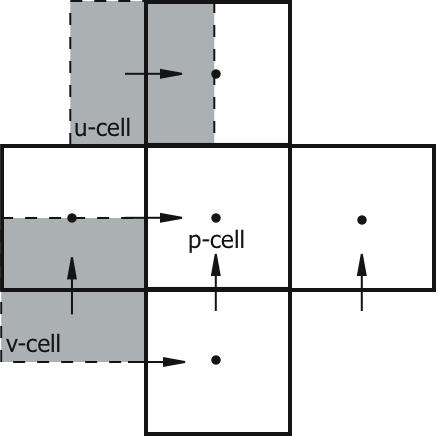
\includegraphics{staggered_grid.png}}
   \caption{Staggered grid arrangement in two dimensions with u and v velocity cell centers located on the face centers of the scalar cells.}\label{fig:staggered_grid}
   \end{center}
\end{figure}
%

The staggering arrangement is advantageous for computing low-Mach LES reacting flows.  First, since a pressure projection algorithm is used, the velocities are exactly projected without interpolation error because the location of the pressure gradient coincides directly with the location of the velocity storage location. Second, Morinishi et al. \cite{morinishi98} showed that kinetic energy is exactly conserved when using a central differencing scheme on the convection and diffusion terms without a subgrid model and in combination with a staggered grid.  Having a spatial scheme that conserves kinetic energy is advantageous because it limits artificial dissipation that arises from the differencing scheme.  These conservation properties make the staggered grid a prime choice for LES reacting flow simulation.

For the spatial discretization of the LES scalar equations, flux limiting and upwind schemes for the convection operator are used.  These schemes are advantageous for ensuring that scalar values remain bounded.  For the momentum equation, a central differencing scheme for the convection operator is used.  All diffusion terms are computed with a second order approximation of the gradient.  

When computing the 2d surface filtered field on the faces of the control volume, one is forced to use an interpolation from the 3d volume filtered field.  This approximation is tolerated because computing the 2d surface field is simply not possible with the given grid scheme. % This is a good example of how LES modeling issues and discrete numerics issue intertwine in applied LES modeling.     

%Jennifer edited
An explicit time stepping scheme is chosen.  A general, multistep explicit update for a variable, $\phi$, may be written as, 
%
%===== Explicit Update =====
\begin{eqnarray}\label{eqn:forward_euler}
\phi^0 = \phi^n \; , \nonumber \\
  \phi^{(i)} = V \sum_{k=0}^{m-1}
\left( \alpha_{i,k}  \phi^{(k)} +
\Delta t \beta_{i,k} L( \phi^{(k)}) \right) \; , \; \; \; \; i = 1, ..., m \\
\phi^{(m)} = \phi^{n+1} \; , \nonumber
\end{eqnarray}
%
where $n$ is the time level, $m$ is the substep between $n$ and $n+1$, $\alpha$ and $\beta$ are integration coefficients, and $L$ is a linearization operator on the the convective flux and source terms.
%
Letting $m=1$ and $\alpha = \beta = 1$ the forward-Euler time
integration scheme is determined,
%%
%%===== Forward Euler =====
\begin{equation}\label{eqn:forward_euler}
\left(  \phi \right)^{n+1} = \left(
\phi \right)^{n} + \Delta t (L( \phi)^n) \; .
\end{equation}
%%
A higher order, multistep method is derived by letting $m > 1$ and
choosing appropriate constants for $\alpha$ and $\beta$. For this
study, two step and three step, strong stability preserving (SSP)
coefficients were chosen from Gottlieb et al.
\cite{Gottlieb75}.

Using the coefficients given by Gottlieb et al., the SSP-RK 2 stepping scheme is
%%
%%===== second order time stepping =====
\begin{eqnarray}\label{eqn:rk_second_order}
( \phi)^{(1)} = ( \phi)^{n} + \Delta
t (L(\phi)^n) \\ \nonumber
( \phi)^{n+1} = \frac{1}{2}(
\phi)^{n} + \frac{1}{2}( \phi)^{1} +
\frac{1}{2}\Delta t (L( \phi)^{(1)}) \;.
\end{eqnarray}
%%
SSP-RK 3 time stepping scheme is,
%%
%%===== third order time stepping =====
\begin{eqnarray}\label{eqn:rk_second_order}
(\phi)^{(1)} = (\phi)^{n} + \Delta t (L(\phi)^n) \\ \nonumber
(\phi)^{(2)} = \frac{3}{4}(\phi)^{n} + \frac{1}{4}( \phi)^{(1)} +
\frac{1}{4}\Delta t (L( \phi)^{(1)}) \\ \nonumber ( \phi)^{(n+1)} =
\frac{1}{3}(\phi)^{n} + \frac{2}{3}(
\phi)^{(2)} + \frac{1}{4}\Delta t (L(
\phi)^{(2)}) \; .
\end{eqnarray}
%%

The time step is limited by
%
\begin{equation}
\Delta t \leq c \Delta t_{F.E.}
\end{equation}
%
where $\Delta t_{F.E.}$ is the forward-Euler time step limited by
the Courant-Friedrichs-Levy condition and $c$ is a constant less
than or equal to one.  

A higher order, multistep method is derived by letting $m > 1$ and choosing appropriate constants for $\alpha$ and $\beta$. For this study, two step and three step, strong stability preserving (SSP) coefficients were chosen from Gottlieb et al. \cite{Gottlieb75}.  The coefficients for SSP-RK 2 and SSP-RK 3 are optimal in the sense that the scheme is stable when $c=1$ if the forward-Euler time step is stable for hyperbolic problems.  In practice, for the Navier-Stokes equations, the value of $c$ is taken less than one.

Choosing an explicit time stepping scheme, rather than an implict one, creates a challenge for solving the set of equations.  The density at the $n+1$ timestep, which is required to determine the cardinal variables,  requires an estimation.  Taking the estimated density for  $\overline{\rho}^{n+1}$ to be $\overline{\rho}^*$, the estimation can be as simple as $\overline{\rho}^* = \overline{\rho}^n$.  Note that the 2d and 3d filter distinction is dropped for the remainder of this discussion for the sake of simplicity.  A slightly more complicated procedure involves a forward-Euler step of the continuity equation to obtain $\overline{\rho}^*$.  This is written as,  
%
\begin{equation}\label{eqn:rho_update}
\overline{\rho}^{ *} = \overline{\rho}^{ n} - \Delta t \frac{S_k}{V} n_{kj} \left(  \overline{\rho} \widetilde{u_j} \right) \; .
\end{equation}
%

% FIXME: section reference is broken
Ideally, one would like to know $\overline{\rho}^{n+1}$ rather than an estimate.  While more details will be discussed in Section \ref{sec:combust_react_models}, one recognizes that $\rho$ is a function of the same variables that are being updated in time, namely, the mixture fraction, $f$, and enthalpy, $h$.  This quandary is a result of the explicit time stepping method will not be resolved for variable density flows without using a fully implicit method.  Explicit methods, however, do have advantages, especially for large scale parallel computations.  Specifically, explicit methods are easier to load balance because the amount of work required for each processor is readily determined a priori, which makes for an efficient parallel computation.  Explicit methods are also easier to code into a computer and to debug.  For these reasons, the current algorithm discussion is limited to explicit methods only. 

The explicit algorithm for solving the set of filtered equations is shown in Algorithm \ref{alg:LES_algorithm}.  
%
%\begin{lstlisting}[float, caption = Explicit LES algorithm, label=alg:LES_algorithm]
%for t:=t_{min} to t_{max} do 
%fill in later..
%for $RK_{step}$:=1 to $N$
%end;
%end; 
%\end{lstlisting}
%
\begin{algorithm}[t]
\caption{Explicit LES algorithm.}\label{alg:LES_algorithm}
%
\begin{algorithmic}[] %add [1] for #'s
\FOR{$t = t_{min}...t_{max}$}
\FOR{$RK_{step} = 1$...$N$} 
\STATE 	Solve for scalars products $(\overline{\rho} \widetilde{f})^{n+1}$ and $(\overline{\rho} \widetilde{h})^{n+1}$.
\STATE	Estimate $\overline{\rho}^* = \overline{\rho}^{n+1}$ from Equation \ref{eqn:rho_update}
\IF{$\overline{\rho}^* < \overline{\rho}_{min}$ or $ \overline{\rho}^* > \overline{\rho}_{max}$}
\STATE $\overline{\rho}^* = \overline{\rho}^{n}$
\ENDIF
\STATE Compute $\widetilde{f}^{n+1} = (\overline{\rho}\widetilde{f})^{n+1}/{\overline{\rho}^*}$ and $\widetilde{h}^{n+1} = (\overline{\rho}\widetilde{h})^{n+1}/{\overline{\rho}^*}$ 
\STATE Compute $\overline{\rho}^{n+1} = f(\widetilde{f}^{n+1}, \widetilde{h}^{n+1})$
\STATE Compute $\widetilde{\mathbf{u}}^*$, the unprojected velocities
\STATE Perform RK averaging if needed
\STATE Compute correct pressure from pressure poisson equation
\STATE Project velocities with correct pressure to get $\widetilde{\mathbf{u}}^{n+1}$ 
\ENDFOR
\ENDFOR
\end{algorithmic}
\end{algorithm}


\subsection{Direct Quadrature Method of Moments}\label{sec:DQMOM}

The direct quadrature method of moments (DQMOM) is a recently-developed moment method for tracking distributions.  It has been applied to distributions of evaporating droplets, soot particle distributions, fluidized beds, and subgrid chemistry PDFs. The method is similar to the quadrature method of moments (QMOM), in that it uses quadrature to provide closure for the moment transport equation; however, it differs in that the moment transport equations are not actually solved, unlike the quadrature method of moments (QMOM). Rather, the DQMOM tracks the quadrature weights and weighted abscissas representing the NDF directly, rather than using the product-difference algorithm to transform between a set of moments and quadrature weights and abscissas that would best represent that distribution.

The basic outline of the method, given below, defines and covers these fundamental steps and concepts:
\begin{enumerate}
\item Number Density Function (NDF)
\item Moments
\item Moment Methods for NDF Transport
\item Quadrature
\item Direct Quadrature Method of Moments
\end{enumerate}

The number density function is the starting point, as it is the function of interest that is being tracked.  Moments are defined, and moment methods are explained and applied to the NDF transport equation to yield the moment transport equation.  Furthermore, quadrature is defined and applied to approximate the moments, which leads to a quadrature-approximated moment transport equation.  This equation leads to the fundamental equations governing DQMOM.

\subsubsection{Number Density Function}\label{subsubsec:NDF}
Using the direct quadrature method of moments (DQMOM) in Arches, the dispersed phase is represented as a number density function (NDF), which is tracked in a stationary Eulerian reference frame. 
The NDF is denoted as $f$ and represents the number of particles at a particular point in space and time.  
Using DQMOM, this NDF is parameterized on several different variables - independent variables for the particles. 
These are called ``internal coordinates,'' and are denoted by $\boldsymbol{\xi}$ (where boldface denotes a vector quantity). 
In this case the NDF is written as $f\left(\boldsymbol{\xi};\boldsymbol{x},t\right)$.

The starting point for the DQMOM equations is the NDF transport equation; this is derived in several places and will not be derived here. The NDF transport equation is:
\begin{eqnarray}\label{eq:NDF transport equation}
  \dfrac{\partial f \left( \boldsymbol{\xi}; \boldsymbol{x},t \right)}{\partial t}  % accumulation term
  + \dfrac{\partial}{\partial x_{i}} \left( \left< u_{i} \vert \boldsymbol{\xi}; \boldsymbol{x}, t \right> f \left( \boldsymbol{\xi}; \boldsymbol{x},t \right) \right) & & \nonumber \\ % spatial convection term
  + \dfrac{\partial}{\partial \xi_{j}} \left( \left< G_{j} \vert \boldsymbol{\xi};\boldsymbol{x}, t \right> f \left( \boldsymbol{\xi}; \boldsymbol{x},t \right) \right)   % phase-space convection term
  & = & h \left( \boldsymbol{\xi}; \boldsymbol{x},t \right),
\end{eqnarray}

\noindent where $G_{j}$ is the velocity of the NDF in phase-space (that is, internal coordinate-space), and is defined by:
\begin{equation}
G_{j} = \dfrac{ d \xi_{j} }{d t}
\end{equation}

\noindent (note this is analogous to spatial velocity $v$, defined by:
\begin{equation}
v_{i} = \dfrac{ d x_{i} }{d t},
\end{equation}

\noindent and that $G_{j}$ takes the same form as Lagrangian particle models); also, $h$ is a birth and death term representing the appearance or disappearance of particles within the domain.  Note also that the velocities $v_i$ and $G_j$ are conditioned on the value of the internal coordinates, as well as on space and time. This implies that the spatial and phase-space velocities are full distributions in $\left( \boldsymbol{\xi}, \boldsymbol{x} \right)$ space, just as the NDF is.

The number of internal coordinates is denoted by $N_{\xi}$. If $N_{\xi} = 1$, the NDF is called ``univariate''; if $N_{\xi} > 1$, then the NDF is called ``multivariate''.



\subsubsection{Moments}\label{subsubsec:moments}
Using DQMOM, the particles are represented as an Eulerian distribution - that is, the particles are not treated in an individual sense, but in a statistical sense. In order to represent the NDF in the framework of a scalar CFD code, the NDF must be represented using a set of scalars that can be transported. One such set of scalars, the moments of the NDF, provide useful statistical information about the distribution. Additionally, a distribution can be approximately reconstructed from its moments. The first moment of the distribution represents the mean value; the second, the variance of the distribution; and so on. An arbitrary number of moments can be defined. For a univariate NDF, the $k^{th}$ moment of the NDF is defined as:
\begin{equation}\label{eq:univariate moment definition}
m_{k} = \dfrac{ \displaystyle{ \int_{-\infty}^{+\infty}{\xi^k f \left( \xi ; \boldsymbol{x},t \right) d\xi } } }{ \displaystyle{ \int_{-\infty}^{+\infty}{ f \left( \xi ; \boldsymbol{x},t \right) d\xi } } }
\end{equation}

Alternatively, if the NDF is a function of several internal coordinates, the $\boldsymbol{k}^{th}$ moment is defined as:
\begin{eqnarray}\label{eq:multivariate moment definition}
m_{\boldsymbol{k}} & = & \dfrac{ \displaystyle{ \dotsintop_{\infty}^{+\infty}{ \xi_{1}^{k_1} \dots \xi_{N_{\xi}}^{k_{N_{\xi}}}   f \left( \xi_1, \dots, \xi_{N_{\xi}} \right)   d\xi_1 \dots d\xi_{N_{\xi}} } }}
{  \displaystyle{ \dotsintop_{\infty}^{+\infty}{ f \left( \xi_1, \dots, \xi_{N_{\xi}} \right)   d\xi_1 \dots d\xi_{N_{\xi}} } } }
%m_{\boldsymbol{k}}  & = & \dfrac{ \displaystyle{ \dotsintop_{-\infty}^{+\infty} \xi_{1}^{k_1} \dots \xi_{N_{\xi}}^{k_{N_{\xi}}}   f \left( \xi_1, \dots \xi_{N_{\xi}} \right)   d\xi_1 \dots d\xi_{N_\xi} }{ \displaystyle{ } }
%				& = & 
\\
m_{\boldsymbol{k}} & = & \dfrac{{\displaystyle \dotsintop_{-\infty}^{+\infty}}\left[
\left({\displaystyle \prod_{m=1}^{N_{\xi}}}\xi_{m}^{k_{m}}\right)
\, f(\boldsymbol{\xi};\boldsymbol{x},t)\, d\boldsymbol{\xi}\right]}{{\displaystyle \dotsintop_{-\infty}^{+\infty}}\, f(\boldsymbol{\xi};\boldsymbol{x},t)\, d\boldsymbol{\xi}}
\end{eqnarray}

\noindent where $\boldsymbol{k} = \left[ k_1, k_2, \dots k_{N_{\xi}} \right] $ is the multivariate moment index.



\subsubsection{Moment Methods for NDF Transport}\label{subsubsec:momentmethods}

The method of moments is a method of tracking the NDF of a system of particles. Because the NDF is a full, continuous distribution, it is difficult to track without assuming a functional form for it. Rather than assume a functional form, the moments of the NDF, which are simply scalars, are tracked instead. This method requires tracking various scalars, which is computationally feasible in a scalar framework and which greatly simplifies the process of tracking the NDF. However, the approach has a closure problem that prevents it from being used in practice for any but the most simple systems.

The transport equation for each moment must be written in terms of higher order moments, and the transport equations for these higher order moments must be written in terms of successively higher order moments, etc. Simplifications (models) must be used to express higher order moments only in terms of lower order moments being tracked as a part of the method of moments. Once this is accomplished, the set of moment transport equations becomes a closed set of equations.



\subsubsection{Quadrature}\label{subsubsec:quadrature}

Quadrature approximates the integral of an unknown function with tabulated known values as a summation of a set of $N$ weighted abscissas. It determines a polynomial of degree $2N-1$ whose zeros are the $N$ weighted abscissas, and approximates the unknown function using this polynomial [Press 1992]. There are several common quadrature formulations, including the midpoint rule (the unknown function is assumed to be a constant, or zero-order polynomial), the trapezoid rule (the unknown function is assumed to be a straight line, or first-order polynomial), and Simpson's rule (the unknown function is assumed to be a second-order polynomial). Note that while the unknown function does not have to be a polynomial, the quadrature approximation becomes much better if it is (and exact if the unknown function is a polynomial of degree $2N-1$ or less). The general $N$-point quadrature formula can be written as:

\begin{equation}\label{eq:quadrature-definition}
\int_{a}^{b}w(r)g(r)\, dx\approx{\displaystyle \sum_{\alpha=1}^{N}w_{\alpha}g(r_{\alpha})}
\end{equation}

\noindent where $g(r)$ is an arbitrary function of the variable $r$. As $N$ increases, the quadrature approximation usually becomes more accurate. This equation can also be extended to a multivariate function $g(\mathbf{r)}$, an arbitrary function of the $D$-element vector $\mathbf{r}=\left[r_{1},r_{2},\dots,r_{D}\right]$ to yield:

\begin{equation}\label{eq:multivariate-quadrature-definition}
{\displaystyle \int_{a}^{b}w(\mathbf{r})g(\mathbf{r)}d\mathbf{r}}
\end{equation}

The weights are common to all internal coordinates $\mathbf{r}$ because the weight function $w(\mathbf{r})$ is binned into $N$ discrete weights, and this weight function is common to all internal coordinates.



\subsubsection{Quadrature-Approximated Moment Transport Equation}\label{subsubsec:quadapproximated}

When the quadrature approximation is applied to a multivariate NDF (where the NDF is the weight function), it yields:

\begin{eqnarray}\label{eq:quadrature-approximated-ndf}
f(\boldsymbol{\xi};\mathbf{x},t) 
& \approx & {\displaystyle \sum_{\alpha=1}^{N}\left(w_{\alpha}(\boldsymbol{x},t){\displaystyle \,\boldsymbol{\delta}\left(\boldsymbol{\xi}-\left\langle \boldsymbol{\xi}(\boldsymbol{x},t)\right\rangle _{\alpha}\right)}\right)} \nonumber \\
& \approx & {\displaystyle \sum_{\alpha=1}^{N}\left(w_{\alpha}(\boldsymbol{x},t){\displaystyle \prod_{j=1}^{N_{\xi}}\delta\left(\xi_{j}-\left\langle \xi_{j}(\boldsymbol{x},t)\right\rangle _{\alpha}\right)}\right)}
\end{eqnarray}

\noindent which makes the integral of the NDF:

\begin{eqnarray}\label{eq:quadrature-approximated-ndf-integral}
{\displaystyle \int_{-\infty}^{+\infty}}\boldsymbol{\xi}^{\boldsymbol{k}}f\, d\boldsymbol{\xi}
&\approx&{\displaystyle \sum_{\alpha=1}^{N}\left\{ w_{\alpha}\left(\prod_{j=1}^{N_{\xi}}\langle\xi_{j}\rangle_{\alpha}^{k_{j}}\right)\right\} }
\end{eqnarray}

This quadrature-approximated NDF can then be substituted into the moment definition to get a quadrature-approximated moment,

\begin{equation}\label{eq:quadrature-approximated-moment}
m_{\boldsymbol{k}}\approx\sum_{\alpha=1}^{N}\left\{ p_{\alpha}\left(\prod_{j=1}^{N_{\xi}}\langle\xi_{j}\rangle_{\alpha}^{k_{j}}\right)\right\} 
\end{equation}

\noindent where $p_{\alpha}$ is the probability of environment $\alpha$ (defined as $w_{\alpha} / \sum_{i=1}^{N} w_{i} $), $\boldsymbol{k}$ is the multivariate moment index vector, and $k_{j}$ is the $j^{th}$ element of vector $\boldsymbol{k}$ (with a total of $N_{\xi}$ values).

Starting with the NDF transport equation, the moment transform can be taken, yielding the moment transport equation. Next, the quadrature approximation can be plugged in, which yields the quadrature-approximated moment transport equation.  After some algebraic manipulation, this yields:

\begin{multline}\label{eq:quadrature-approximated-moment-xport-eqn}
{\displaystyle {\displaystyle \sum_{\alpha=1}^{N}\left[
{\displaystyle \prod_{j=1}^{N_{\xi}}}\delta\left(\xi_{j}-\left\langle \xi_{j}\right\rangle _{\alpha}\right)
+\sum_{m=1}^{N}\dfrac{\partial}{\partial\langle\xi_{m}\rangle_{\alpha}}\left(\prod_{j=1}^{N_{\xi}}
\delta\left(\xi_{j}-\left\langle \xi_{j}\right\rangle _{\alpha}\right)
\right)\langle\xi_{m}\rangle_{\alpha}\right]}a_{\alpha}} \\
-\sum_{\alpha=1}^{N}\sum_{n=1}^{N}\left[\dfrac{\partial}{\partial\langle\xi_{n}\rangle_{\alpha}}\left(\prod_{j=1}^{N_{\xi}}
\delta\left(\xi_{j}-\left\langle \xi_{j}\right\rangle _{\alpha}\right)
\right)\right]b_{n\alpha}= \\
{\displaystyle \sum_{\alpha=1}^{N}\sum_{m=1}^{N_{\xi}}\sum_{n=1}^{N_{\xi}}}\left[\dfrac{\partial^{2}}{\partial\langle\xi_{m}\rangle_{\alpha}\partial\langle\xi_{n}\rangle_{\alpha}}\left({\displaystyle \prod_{j=1}^{N_{\xi}}
\delta\left(\xi_{j}-\left\langle \xi_{j}\right\rangle _{\alpha}\right)
}\right)\right]C_{mn\alpha} \\
+S_{\xi}+D_{\xi}+h,
\end{multline}

\noindent where $a_{\alpha}$ and $b_{n,\alpha}$, defined as:

\begin{eqnarray}\label{eq:a-b-transport-eqns}
\dfrac{\partial}{\partial t}\left( w_{\alpha} \right)
+\dfrac{\partial}{\partial x_{i}}\left( \langle u_{i}\rangle_{\alpha}w_{\alpha} \right)
-\dfrac{\partial}{\partial x_{i}} \left( D_{x,\alpha} \dfrac{\partial}{\partial x_{i}} \left( w_{\alpha} \right) \right)
&=&a_{\alpha} \\
\dfrac{\partial}{\partial t}\left( \varsigma_{n\alpha} \right)
+\dfrac{\partial}{\partial x_{i}}\left( \langle u_{i}\rangle_{\alpha}\varsigma_{n\alpha} \right) 
-\dfrac{\partial}{\partial x_{i}}\left( D_{x,\alpha} \dfrac{\partial}{\partial x_{i}} \left( \varsigma_{n,\alpha} \right) \right) 
&=&b_{n\alpha}, \\
&&\nonumber \\ 
\text{for }j=1\dots N_{\xi} & & \nonumber
\end{eqnarray}

\noindent are the transport equations implemented to track the evolution of the NDF.  The source terms $a_{\alpha}$ and $b_{n,\alpha}$ come from the solution to the linear system

\begin{equation}\label{eq:Ax=B}
\mathbf{Ax} = \mathbf{B}.
\end{equation}

\subsubsection{Build of Ax=B}\label{subsubsec:buildAX=B}
There are $N_e(N+1)$ unknowns for $a_a$ and $b_{na}$, while there
are just one linear equations for them. In order to build a complete
linear system, $N_e(N+1)-1$ moments are needed. And DQMOM method
is used to build this linear system. Using properties of delta functions,
the $k^{th}$ moment for Eq.(\ref{eq:a-b-transport-eqns}) is derived
as



\begin{equation}
\begin{split}
\sum_{a=1}^{N_{e}}\left[\left(\prod_{n=1}^{N}\left<\xi_{n}^{k_n}\right>_{a}\right)-\sum_{m=1}^{N}k_m\left(\left<\xi_{m}^{k_m}\right>_{a}\right)\left(\prod_{n=1,n\neq m}^{N}\left<\xi_{n}^{k_n}\right>_\alpha\right)\right]a_{a}
\\
+\sum_{a=1}^{Ne}\sum_{n=1}^{N}\left[k_n\left<\xi_{n}^{k_n-1}\right>_{a}\left(\prod_{m=1,m\neq n}^{N}\left<\xi_{m}^{k_m}\right>_{a}\right)\right]b_{a,n}=
\\
\sum_{a=1}^{Ne}\sum_{m=1}^{N}\left[k_m\left(k_m-1\right)\left<\xi_m^{k_m-2}\right>_a\times\left(\prod_{j \neq m,j=1}^{N_\xi}\left<\xi_j^{k_j}\right>_a\right)\right]{w}_a{C}_{mma}+
\\ \sum_{a=1}^{Ne}\sum_{m=1}^{N}\sum_{n=1}^{N}\left[k_mk_n\left<\xi_{m}^{k_m-1}\right>_{a}\left<\xi_n^{k_n-1}\right>_a\times\left(\prod_{j=1,j \neq m}^{N}\left<\xi_{j}^{k_j}\right>_{a}\right)\right]w_{a}C_{mna}+\bar{S}_{k}+\bar{D}_{k}
\end{split}
\label{eq:kth_moment}
\end{equation}

and

\begin{equation}
\bar{S}_{k}=-\sum_{a=1}^{N_{e}}\sum_{n=1}^{n}\left[\left(\prod_{m=1,m\neq n}^{N}\left<\xi_{m}^{k_{m}}\right>\right)\left(k_{n}\left<\xi_{n}^{k_{n}-1}\right>_{a}\right)\left(w_{a}\left<G_{n}\right>_{a}\right)\right]
\end{equation}


\begin{equation}
\bar{D}_{k}=\sum_{a=1}^{N_{e}}\sum_{n=1}^{n}\left(\prod_{m=1,m\neq n}^{N}\left<\xi_{m}^{k_{m}}\right>_{a}\right)\left(k_{n}\left(k_{n}-1\right)\left<\xi_{n}^{k_{n}-2}\right>\right)\left(w_{a}\Gamma_{\xi_{n},a}\right)\label{eq:Dk_bar}
\end{equation}


where $k_m$ represent the $k^{th}$ moment for the $m^{th}$ internal
coordinates. With a reasonable selection of the moments for each internal
coordinates, a linear system with a rank of $N_e\left(N+1\right)$
can be constructed by

\begin{equation} \label{eq:AXeqB1}
[A_{1},A2]*[a_{a},b_{an}]^{\textrm{T}}=[C_{k}+\bar{S}_{k}+\bar{D}_{k}]^{\textrm{T}}
\end{equation}

\subsubsection{solution of DQMOM matrix} \label{subsubsec:solutionax=b}
The detailed solution method can be find in Charles and Julien's Thesis \cite{Charles_DQMOM, Julien_thesis}. The typical LU solution will offten met singular problems, so Rodney provided a method to rebuild matrix A and B to avoid this problem\cite{RF_2009}. This method is named as "Optimize" in <DQMOM> block. However, the "Optimize" method is very time consuming.

\subsubsection{Simplest method in DQMOM} \label{subsubsec:Simplest}
In order to save CPU times for DQMOM method, some simplified method can be adopted to define the source term for \ref{eq:a-b-transport-eqns}, or $X$. For coal combustion case, when the following assumption was adopted
\begin{itemize}
\item Assuming that any scalars distribution of the coal particles can be
perfectly represented by multi-delta functions, especially, the particle
velocity distribution can be perfectly represented by $\left<v_{a}\right>$,
so that there is no diffusion terms. In other words, the third term
at the right side and $D_\xi$ in Eq.(\ref{eq:AXeqB1}),
are omited. This is only correct for each single particle, so that
integral of Eq.(\ref{eq:quadrature-approximated-moment-xport-eqn}) with a
moment becomes the Langrangian particle equations as:
\end{itemize}
\begin{equation}
\frac{d\xi^{m}}{dt}=S_{\xi^{m}}
\end{equation}

where $\xi^m$ is the moment that we are interested. As long as we
consider a reprentative particles for a group of particles, such diffusion
term will exists, which are hard to be modeled. A reasonable way to
eliminate the effect of diffusion term is to increase the phase numbers.
(but this will meet other chanllenges, for e.g., for the dense phase,
the interactions between two phases need to be considered, the computation
cost would be hudge).
\begin{itemize}
\item For pulverized coal combustion system, the particles are very dispersed,
so that any particle-particle interactions is small enough (comparing
partile-gas interactions) to be omited. With this assumption, the
source term, $S_\xi$ can be easily represented by the single particle
models, so that Langrangian style models can be used.
\item There is no particle death or birth, so that the weights do not change
with the internal coordinates $\xi$. In other words, $a_a$ in Eq.(\ref{eq:a-b-transport-eqns})
equals to 0 and the rank of the linear system is reduced from $N_e(N+1)$
to $N_eN$.
\end{itemize}
Taking these three assumptions, the linear system can be reduced further,
since there is no diffusion terms, the right side of Eq.(ref\{eq:kth\_moment\})
is reduced to $\bar{S}_k$. Then we just consider the first moments
for $\xi_{n,a}$ and $0^{th}$ moments for other $\xi$(let $k_n=1, and k_(m\neq n)=0$
for the $p^{th}$ phase. This makes the linear system, Eq.(\ref{AXeqB})
reduces to

\begin{equation}
0+\ldots+\text{0+}b_{n,a}+0+\ldots0=w_{a}\left<G_{n}\right>_{a}=w_{a}\frac{d\xi_{n,a}}{dt}
\end{equation}


That means the linear system is already solved without any further
calculations (no need of solving linear systems). and the transport
equations of the weights and weighted abscissas finally are simplified
to

\begin{equation}
\frac{\partial}{\partial t}\left(w_{a}\right)+\frac{\partial}{\partial x_{i}}\left(\left<v_{i}\right>_{a}w_{a}\right)=0\label{eq:ap_transport-simple}
\end{equation}


\begin{equation}
\frac{\partial}{\partial t}\left(\zeta_{n,a}\right)+\frac{\partial}{\partial x_{i}}\left(\left<v_{i}\right>_{a}\zeta_{n,a}\right)=w_{a}\frac{d\xi_{n,a}}{dt}\label{eq:simplified_transport_equation}
\end{equation}


It should be noted these are instantaneous equations, and SGS model
should be considered for LES simulation. If we know the diffusion
models, and just with no birth/dirth of particles. There are also
no need to solve the transport equations, if only the internal coordinates
are independent, or if we can build the direct correlation among these
dependent moments. For e.g., if we have to consider the particle surface
and the particle diameter as well as the particle volume, these internal
coordinates are correlated, and linear system is needed to be built
for such dependent moments if the particle diameter, surface and volume
change can't be decribed by three separate models. For the coal combustion
systems we are considering, the internal coordinates are independent,
so there is no need to solve the linear system. and the final transport
equations are

\begin{equation}
\frac{\partial}{\partial t}\left(w_{a}\right)+\frac{\partial}{\partial x_{i}}\left(\left<v_{i}\right>_{a}w_{a}\right)+\frac{\partial}{\partial x_{i}}\left(D_{x,p}\frac{\partial}{\partial x_{i}}\left(w_{a}\right)\right)=0\label{eq:ap_transport-simp_diffusion}
\end{equation}


\begin{equation}
\frac{\partial}{\partial t}\left(\zeta_{n,a}\right)+\frac{\partial}{\partial x_{i}}\left(\left<v_{i}\right>_{a}\zeta_{n,a}\right)+\frac{\partial}{\partial x_{i}}\left(D_{x,a}\frac{\partial}{\partial x_{i}}\left(\zeta_{n,a}\right)\right)=w_{a}\frac{d\xi_{n,a}}{dt}+D_{\xi_{n,a}}\label{eq:simplified_transport_equation_with diffusion}
\end{equation}


The chanllenge is that $D_{x,a}$ and $D_{\xi_{n,a}}$ almost can't
be modeled (seems $D_{\xi_{n,a}}=0$ when multi-delta functions adopted, according to Eq.(\ref{eq:Dk_bar}).
and we'd rather to consider more phases to elimate the diffusion terms. 



Taking the assumptions mentioned above, the transport equations of
PBE in form of PDF acutally degenerate to multi-phase Euler-Euler
equations without consideration phase-phase interactions (except for
gas-particle interactions). If the particle phase are enough so that
each particle is represented by a phase, Eq(\ref{eq:ap_transport-simple})
and Eq(\ref{eq:simplified_transport_equation_with diffusion}) are
actually Lagrangian method. Or in other words, the simplest case we
adopted with DQMOM method equvalent that we are using Lagrangian method
to track infinitely large number of particles falling to only $Ne$
categories (each categories of particle has the same values for all
$N$ internal coordinates). 




\subsubsection{Summary}\label{subsubsec:summary}
In summary, the DQMOM solution procedure requires solving several transport equations, given by \ref{eq:a-b-transport-eqns}. These transport equations describe the changes in the quadrature weights and weighted abscissas used to approximate the NDF.  The source terms for these transport equations, $a_{\alpha}$ and $b_{n,\alpha}$, come from the solution to a linear system, $\mathbf{Ax}=\mathbf{B}$, in which the vector $\mathbf{x}$ contains the source terms.  This linear system comes from the quadrature-approximated moment trasport equation, equation \ref{eq:quadrature-approximated-moment-xport-eqn}, of which there are $\left(N_{\xi} + 1\right)N$.  It is because this set of equations is linear in the unknowns $a_{\alpha}$ and $b_{n,\alpha}$ that it can be re-cast in the form of a linear system.

\subsection{Wall Heat Transfer Model in Arches} \label{subsec:WHT}
\subsubsection{Basic assumptions and models for wall heat transfer}

The basic assumptions are as follows:
\begin{itemize}
\item Wall is regarded as black body, the heat released by the wall is calculated
by Stefan-Boltzmann law, this assumption is consistant to the assumption
adopted in DO radiation method in ARCHES.
\item There is no time derivation term for wall heat transfer, in other
words, wall temperature comes to equilibrium state instantaneously
at each time step. While a relaxation coefficient, $C_{rex}$, is
adopted to smooth the wall temperature change, or $T_w=(1-C_{rex})T_{w0}+C_{rex}T_w$.
\item When considering convection heat transfer, the gas temperature is
represent by the Cell-Center gas temperature adjecent to the wall,
Pr and Re is calculated based on the velocities and properties of
the CC value adjecent to the wall. But up to now, no convection heat
transfer is considered in ARCHES.
\item thermal resistance from fluid to the tubes is small enough to be neglected,
so that inside tube wall temperature is set to a constant value. (<tube\_side\_T>
in arches.spec)
\end{itemize}
The wall heat transfer is calculated by

\begin{equation}
q_{net}=(T_{w}-T_{in})/R_{wc}\label{eq:wallht}
\end{equation}


\begin{equation}
q_{net}=\epsilon_{w}(q_{in}-q_{rad\_w})+q_{conv}\label{eq:net}
\end{equation}


where $q_{net}$ is the heat flux absorbed by the wall. $q_{in}$
is the incidental radiation heat flux from the ambient gas phase to
the wall surface, which is provided by radiation solver in ARCHES,
$q_{rad\_w}$ is the heat flux of the black-body wall emission, and
can be calculated by

$q_{rad\_w}=\sigma T_{w}^{4}$

$q_{conv}$ is the heat flux absorbed by the wall through convection,
$T_w$ and $T_{in}$ are the wall surface temperature (represented
by 'temperature' in ARCHES simulation) and fluid temperature inside
wall tubes (<tube\_side\_T>), and $R_{wc}$ is the wall thermal resistance,
$R_{wc}=l/\lambda$, $l$ is the <wall\_thickness> in areches.spec,
and $\lambda$ is <k> in arches.spec.


\subsubsection{Algorithms of wall heat transfer solution in Arches\label{sec:Algorithms-of-wall}}

Eq.\ref{eq:wallht} can be recasted by

\begin{equation}
T_{w}=T_{in}+q_{net}R_{wc}\label{eq:3}
\end{equation}


Based on Eq.\ref{eq:3}, an iterative algorithm was proposed to solve
$T_w$:
\begin{enumerate}
\item Taking an initial $T_w$ and calculate $q_{net}$ by Eq.(\ref{eq:net}) 
\item Calculate $T_w$ by Eq.\ref{eq:3}. And return back to Step.1
\end{enumerate}
Since $q_{net}$ is sensitive to $T_w$ due to Stefan-Boltzmann law,
this iteration method is unstable and it's hard to get the final resolutions.
So an relaxation coefficient was introduced to help converge. Then
the final iteration method would be
\begin{enumerate}
\item calculate $q_{net}$ based on $T_{w0}$ by Eq.\ref{eq:wallht}
\item Calculate $T_{w1}$ with Eq.\ref{eq:3}
\item Calculate renewed $T_{w1}$ by $T_{w1}=(1-C_{relx})T_{w0}+c_{relx}T_w'$.
Then go back to step1 with $T_{w1}$
\end{enumerate}
This Relaxation Iteration Method (RIM) can be used to get the final
$T_w$ at each timestep. Although with small Relaxation Coefficient,
RIM method may still be unstable if $R_{wc}$ is very large.

$T_w$ can also be calculated by another iterations method such as
Dichotomy Iteration Method (DIM)as follows:
\begin{enumerate}
\item To set a maximum wall temperatrue $T_{wmax}$ and a minimum wall temperature
$T_{wmin}$.
\item to calculate initial wall temperature $T_{w0}=(T_{wmax}+T_{wmin})/2$
\item To calculate $T_{w1}$ with Eq\ref{eq:wallht}, Eq\ref{eq:net} and
Eq\ref{eq:3}.
\item if $T_{w1}>T_{w0}$, then $T_{wmin}=T_{w0}$; if $T_{w1}<T_{w0}$,
then $T_{wmax}=T_{w0}$. Then go to step.2 to make iteration, till
$T_{w1}-T_{w0}<error$
\end{enumerate}
The advantage of this method is that the iteration won't be oscilate
and will always converge. Given a reasonable initial $T_{wmax}$ and
$T_{wmin}$ (Which are <max\_TW> and <min\_TW> in arches.spec), the
DIM will have very small cost. 

\subsubsection{black body or grey body assumption?}

Up to now, the wall emissivity $\epsilon_{w}$ in Eq.\ref{eq:net}
is set to 1.0 in arches code, since that in DO model, the wall is
assumed to be the black-body. If the grey body assumption has to be
considered, we must make sure that radiation model (DO or RMCRT) also
consider a greybody condition for the wall. Still, there is a trick
to treat the wall as greybody in wall heat transfer model while keep
adopting blackbody assumptions in Radiation model. The trick is as
follows:
\begin{enumerate}
\item take an $\epsilon_{w}$ of less than one in Eq.\ref{eq:net}, and
calculate the grey wall temperature $T_{w1}$ and $Q_{net}$ with
the iteration method mentioned in Section\ref{sec:Algorithms-of-wall}.
\item To modify the wall temperature from $T_{w1}$ to $T_w$,  so that
the following equations are satisfied: $q_{net}=q_{in}-\sigma T_{w}^{4}$.
Generally the difference between $T_w$ and $T_{w1}$ is no more than
20K if $\epsilon_{w}=0.8$. So the emissivity won't change the wall
temperature a lot. However, it will be better if the wall reflection
can be considered in the radiation model.
\end{enumerate}

\subsubsection{numerical steadyness, especially for adiabatic wall BC or small thermal
conductivities}

In Section.\ref{sec:Algorithms-of-wall}, the calculation of $T_w$
is proposed for each times step. During LES simulation, $q_{in}$
will change with $T_w$ as well. The following conditions will cause
the numerical simulation of $T_w$ unsteady
\begin{itemize}
\item A bad initial temperature assumption: a bad initial temperature assumption
will casue a bad initial $q_{in}$, and thus a bad $T_w$, although
$T_w$ is 'accurate' at this timestep, it's a fake wall temperature
and may have negative effect on $q_{in}$ in next step.
\item When simulation case is large and simulation domain is complex, the
previous tests show that the simulation is sentitive to wall temperature.
If $T_w$ changes frequently and changes in a large range, this may
cause some numerical problems in Arches simulation. 
\end{itemize}
with these consideration, it's better to change $T_w$ smoothly when
$q_{in}$ is sensitive to $T_w$. So at the beginning of simulation,
a small relaxation coefficient can be adopted to control the change
of $T_w$. When simulation comes to a steady state, RIM and DIM moethod
can be directly adopted to get the final $T_w$. However, the strategy
of $T_w$ calculation depends on the real physical problems. 

For adiabatic wall boundary conditions, since the thermal resisitance
($R_{wc}$) is infinitly large, numerical steady is a challenge when
we use iterative method to calculate Eq.\ref{eq:3}, and DIM is a
good way to solve this problem. In ARCHES, the DIM method is adopted
and the adiabatic wall will be well solved. Still, a small relaxation
coefficient, $C_{rex}$, is recommend to be adopted. For e.g., $C_{rex}=0.05$,
which will help to acquire a smooth change of wall temperature with
time.






\subsection{Digital Filter Generator for Turbulent Inlet Conditions}\label{sec:DFG}
The digital filter method generates a set of both spatially and temporally correlated random data in order to create a synthetic turbulent inlet.  In the Arches implementation, the data is generated a priori.

\subsubsection{Digital Filter}
Let $r_m$ be a set of random data such that $\left\rangle r_m \right\rangle = 0$ and $\left\lbrace r_m^2 \right\lbrace =1$.  Then there exists a set of filter coefficients $b_n$ for the convolution such that

\begin{equation} \label{eq:DFGconv}
u_m = \sum_{-N}^N b_n r_{m+n}
\end{equation}

where $N$ is the support of the filter. If \ref{eq:DFGconv} is rearranged in the form of an autocorrelation function then it follows that

\begin{equation} \label{eq:DFGauto}
\frac{\bar{u_m u_{m+k} } }{ \bar{u_m u_m }  } = \sum_{j=-N+k}^N b_j b_{j-k} \big/ \sum_{j=-N}^N b_j^2
\end{equation}

For extending filter coefficients to three dimensions a simple convolution of the three one-dimensional filters is used.

\begin{equation} \label{eq:DFG3D}
b_{ijk} = b_i \cdot b_j \cdot b_k
\end{equation}

Now consider a fully developed flow.  A fit line for its autocorrelation function can be expressed as an exponential decay

\begin{equation}
R_{uu} (r) = \exp \left( - \frac{ \pi r^2}{4 L^2} \right)
\end{equation}

where L is the integral length scale. If the grid spacing is $\Delta x$ then the length scale can be set as $L = n \Delta x$, and the discrete autocorrelation function is then

\begin{equation}
R_{uu} ( k \Delta x) = \exp \left( - \frac{ \pi (k \Delta x)^2}{4 (n \Delta x)^2} \right) = \exp \left( - \frac{ \pi k^2}{4 n^2} \right)
\end{equation}

Now apply \ref{eq:DFGauto} to relate the discrete autocorrelation function to the filter coefficients

\begin{equation}
R_{uu} (k \Delta x) = \frac{ \bar{ u_m u_{m+k} } }{ \bar{u_m u_m} } = \sum_{j=-N+k}^N b_j b_{j-k} \big/ \exp \left( - \frac{ \pi k^2}{4 n^2} \right)
\end{equation}

There is an approximate solution to the filter coefficients available

\begin{equation} \label{eq:DFGfiltercoef}
b_k \approx \tilde{b}_k \big/ \left(  \sum_-N^N  \tilde{b}_j^2 \right)^{1/2} \; \; \text{with} \; \; \tilde{b}_k = \exp \left( - \frac{ \pi k^2}{2 n^2} \right)
\end{equation}

which is a valid approximation as long the the filter support is sufficiently large, $N \geq 2n$.  This maintains the the support of the filter is large enough to capture twice the length scale. This is a brief explanation of the method from Klein's paper \cite{Klein2003}. Note that as $ N \rightarrow 0$ this method approaches white noise.

\subsubsection{Implementation Algorithm}
The steps in generating the inlet data are listed here directly from Klein's procedure for isotropic flow \cite{Klein2003}.

\begin{enumerate}
\item Choose a length scale for each coordinate direction as$ L_{y}=n_{y}\Delta y , L_{z}=n_{z}\Delta z $ and a timescale for the flow direction (or length scale by Talyor's hypothesis) $T_{x}=n_{t}\Delta t$  (or $L_{x} = n_x \Delta x$ ), set the size of the support $N_{\alpha}\geq 2n_{\alpha} $ for $\alpha=x,y,z$ . Also prescribe a mean flow profile.
\item Initialize three random fields $\mathcal{R}_{\alpha}$  of dimensions $[-N_{x}:N_{x},-N_{y}+1:M_{y}+N_{y},-N_{z}+1:M_{z}+N_{z} ]$ , with $M_{y}\times M_{z}$  denoting the resolution of the grid of the inflow plane. The size is actually $[2N_{x}+1,2N_{y}+M_{y},2N_{z}+M_{z} ]$.
\item Calculate the filter coefficients b(i,j,k), using \ref{eq:DFGfiltercoef}
\item Loop over the inlet dimensions j  and k  and apply the filter operation for each velocity fluctuation
\begin{equation} \label{eq:DFGmain}
\mathcal{U}_{\alpha}(j,k)=\sum_{i'=-N_{x}}^{N_{x}}\sum_{j'=-N_{y}}^{N_{y}}\sum_{k'=-N_{z}}^{N_{z}}b(i',j',k')\mathcal{R}_{\alpha}(i',j+j',k+k') 
\end{equation}
\item Using the time-averaged Reynold's stress tensor ($R_{ij}$)  solve for the transformation matrix $a_{ij}$
\begin{equation}
 a_{ij}=\left[\begin{array}{ccc}
(R_{11})^{1/2} & 0 & 0\\
R_{21}/a_{11} & (R_{22}-a_{21}^{2})^{1/2} & 0\\
R_{31}/a_{11} & (R_{32}-a_{21}a_{31})/a_{22} & (R_{33}-a_{31}^{2}-a_{32}^{2})^{1/2}
\end{array}\right] 
\end{equation}
\item  Now solve for each of the velocity components
\begin{equation}
u_{i}=\bar{u_{i}}+a_{ij}\mathcal{U}_{j} 
\end{equation}
\item Shift the random data set by the flow direction $\mathcal{R}_{\alpha}(i,j,k)=\mathcal{R}_{\alpha}(i+1,j,k)$ , and fill the last plane $\mathcal{R}_{\alpha}(N_{x},j,k)$  with new random numbers.
\item Repeat steps 4 through 7 for each timestep
\end{enumerate}

In Arches two major changes are made to this algorithm. First the data is all pre generated into a table that is loaded when the simulation starts. This happens because the summation in \ref{eq:DFGmain} can become very expensive at high resolution and occurs at each point in the boundary, and some issues with trying to deal with the random field at patch boundaries. The second is that the option to use Taylor's hypothesis of frozen turbulence is utilized so that the length scale is specified in the flow direction, rather than the time scale. Then the same flow profile is reused for several timesteps, this period is either specified as the number of steps or as a time.


% ==========================================================
% =============== Uintah Specifications =========================
% ==========================================================
\section{Uintah Specification}
%
\subsection{Basic Inputs}
%
Choosing the ARCHES component is done through the simulation controller using the {\it SimulationComponent} tag.  In this case (similar to the other Uintah components) the Arches component is specified as
%
\begin{Verbatim}[fontsize=\footnotesize]
<SimulationComponent type="arches" />
\end{Verbatim}
%
as a child of the \verb=<Uintah_Specification>= section.  

Most other Arches specifications are located in the {\it CFD$\rightarrow$ARCHES} section of the input file.  Unless otherwise specified, the system of units for all Arches input parameters are SGI.

\subsection{Boundary Conditions}\label{sec:boundaryconditions}
Boundary conditions for Arches are specified using the Uintah boundary condition mechanism.  As such, all boundary conditions for domain faces are specified in the \verb=<Grid>=$\rightarrow$\verb=<BoundaryConditions>= section of the input file.  Generic details of the UCF boundary condition mechanism may be found in \ref{sec:ucf_bc}.  

Generally, boundary conditions are required for every transport equation except at periodic boundaries.  Specifically, every equation specified in the \verb=<TransportEqn>= section of the input file requires domain boundary specification on every domain face.  

The generic options for the boundary condition type include \verb=Dirichlet= and \verb=Neumann= conditions.  For the \verb=Dirichlet= condition, transported variables at domain boundaries satisfy the condition, 
%
\begin{equation}
\phi_b = \alpha_D
\end{equation}
%
where $\phi_b$ is the transported variable at the domain extent and $\alpha_D$ is the value specified in the \verb=<BCType>=$\rightarrow$\verb=<value>= tag. The \verb=Neumann= condition specifies the gradient of $\phi$ at the boundary and thus satisfies the condition, 
%
\begin{equation}
\frac{\partial \phi}{\partial n}|_b = \alpha_N
\end{equation}
%
where $n$ is the normal direction of the boundary and $\alpha_N$ is the value specified in the \verb=<BCType>=$\rightarrow$\verb=<value>= tag.  

Momentum boundary conditions are specified using descriptive tags that in turn choose the appropriate Nuemann, Dirichlet, or some other boundary condition depending on the tag.  Note that some momentum boundary conditions have implications for all transported variables despite any previously specified boundary condition for that specific scalar.  This is described below.  

Boundary conditions for momentum include (with the corresponding \verb=<BCTyep var>= attribute listed), 
%
\begin{itemize}
\item Specified velocity inlet (\verb=VelocityInlet=)
\item Specified mass flow rate (\verb=MassFlowInlet=)
\item Specified swirl inlet (\verb=Swirl=)
\item Velocity inlet read from file (\verb=VelocityFileInput=)
\item Digital Filter turbulence inlet from file (\verb=TurbulentInlet=)
\item Pressure boundary condition (\verb=PressureBC=)
\item Outlet boundary condition (\verb=OutletBC=)
\item Wall boundary condition (\verb=WallBC=)
\end{itemize}
%
Details of each boundary condition follow.

\subsubsection*{Velocity Inlet}
%
The velocity inlet specification requires that \verb=<vecvalue>= be specified as a child of \verb=<BCType>=, where \verb=<vecvalue>= represents a three component vector of velocity at the inlet. For example, 
%
\begin{Verbatim}[fontsize=\footnotesize]
<Face circle="x-" radius="0.5" centroid="0 0.5 0.5">
	<BCType var="VelocityInlet" id="0" label="my velocity inlet">
		<vecvalue>[0.1, 0.2, 0.2]</vecvalue>
	</BCType>
</Face>
\end{Verbatim}
%
specifies a non-normal velocity component in a circular region on the x-minus face.  Note that the \verb=label= attribute is generic here, allowing the user to specify any descriptive title to the boundary condition.  

Velocity inlet boundary conditions simply set the velocity vector at domain boundary interface.  To ensure a constant mass flow rate for the given velocity condition, the actual velocity at the domain interface may vary to compensate for varying density within the domain while maintaining a constant mass flow rate into the domain.  This step is necessary because density is a cell centered quantity and interpolation of density to the face may potentially change the mass flow rate if the velocity is not adjusted accordingly.  This is accomplished by computing the following for the normal velocity component, 
%
\begin{equation}
u_{n} = 2.0( \rho u )_{b} / (\rho_{i} + \rho_{b}), 
\end{equation}
% 
where $n$ indicates the normal interfacial velocity, $b$ is the boundary density, and $i$ is the density from the first interior cell in the normal direction of the boundary.  Note that a simple linear interpolant has been used to compute the boundary density.  

\subsubsection*{Mass Flow Inlet}
%
The mass flow inlet boundary condition requires that \verb=<value>= be specified as a child of \verb=<BCType>=, where \verb=<value>= is the mass flow rate in units of \verb=[kg/s]=. For example, 
%
\begin{Verbatim}[fontsize=\footnotesize]
<Face circle="x-" radius="0.5" centroid="0 0.5 0.5">
	<BCType var="MassFlowInlet" id="0" label="my mass flow inlet">
		<value>0.4</value>
	</BCType>
</Face>
\end{Verbatim}
%
specifies a mass flow rate in a circular region on the x-minus face.  Note that the \verb=label= attribute is generic here, allowing the user to specify any descriptive title to the boundary condition.  

A velocity condition is set from the mass flow rate condition using the area and density of the boundary geometry.  Note that the area of the geometry is computed from the true area of assembly of the grid cells and not the ideal geometry area.  Once velocities are computed, the mass flow rate boundary condition proceeds as the previously described velocity inlet condition.  

\subsubsection*{Swirl Inlet}
% 
The swirl condition specifies a mass flow rate condition in addition to adding a swirling component from the non-normal velocity components.  This specification requires that the \verb=<value>= (mass flow rate, \verb=[kg/hr]=), \verb=<swirl_no>= (swirl number), and \verb=<swirl_centroid>= be specified as a child of \verb=<BCType>=.  For example, 
%
\begin{Verbatim}[fontsize=\footnotesize]
<Face circle="x-" radius="0.5" centroid="0 0.5 0.5">
	<BCType var="Swirl" id="0" label="my swirled inlet">
		<value>1.0</value>
		<swirl_no>16.0</swirl_no>
		<swirl_centroid>[0, 0.5, 0.5]</swirl_centroid>
	</BCType>
</Face>
\end{Verbatim}
%
specifies a mass flow inlet in a circular region on the x-minus face with a swirl number of 16 and a centroid coincident with the circle of the boundary geometry.  Note that the swirl condition currently is applied across the entire geometry. 
%
%add brief description of the swirl condition here.....

\subsubsection*{Velocity File Input Inlet}
% 
Work in progress....please check back later. 

\subsubsection*{Turbulent Inlet} \label{subsubsec:TurbInlet}
%
The turbulent inlet loads a pre-generated table consisting of cell indices for each realization time index provided.  It requires a period, which specifies the amount of simulation time to use the same profile, a vector value to set up the iterator, and the input file to load.  An example specification is
%
\begin{Verbatim}[fontsize=\footnotesize]
<Face circle="x-" radius="0.25" origin="0 0.5 0.5">
  <BCType id-"all" var="TurbulentInlet" label="my_turbulent_inlet">
    <value> [1.0, 0.0, 0.0] </value>
    <period> 10 </period>
    <inputfile> tubulent_input_file.gz </inputfile>
  </BCType>    
</Face>
\end{Verbatim}
%
This loads the table and changes the time index of the realization to use once every 10 simulation timesteps.  The period is an optional parameter that defaults to 1. If a timescale is used for generation the period should be one, but if a length scale is used for the flow direction, then the period needs to be such that sufficient time elapses to convect the velocity through one cell.  A \verb=<timeperiod>= specification can also be used, which is more convenient for a variable \verb=dt= problem. The input file needs to have the number of total realizations generated and the non axial dimensions of the box around the inlet in the first line.  The next line needs to be the minimum (i, j, k) cell index of the bounding box of the inlet, all of the indices of the velocity vectors stored are in relation to the corner being at (0, 0, 0), so this adjusts from the simulation's (i, j, k) to match.  Then a list of the (t, j,k) points and (u, v, w) vectors, varying first by k, then j, then t (for a x- or x+ face).  For other faces either (t, i, k) or (t, i, j) points are listed instead.  It is recommended to use the \verb=DigitalFilterGenerator= executable for creating a table.

\subsubsection*{Pressure Boundary Condition}
%
A pressure (open) boundary condition is specified using \verb=PressureBC= attribute.  For example, 
%
\begin{Verbatim}[fontsize=\footnotesize]
<Face side="y+">
	<BCType var="PressureBC" id="0" label="y+ pressure bc"/>
</Face>
\end{Verbatim}
%
specifies a pressure condition on the \verb=y+= face of the domain. 
%
% add brief description of the pressure condition here

\subsubsection*{Flow Outlet Boundary Condition}
%
A flow outlet boundary condition is specified using \verb=OutletBC= attribute.  For example, 
%
\begin{Verbatim}[fontsize=\footnotesize]
<Face side="y+">
	<BCType var="OutletBC" id="0" label="x+ outlet bc"/>
</Face>
\end{Verbatim}
%
specifies an outlet condition on the \verb=x+= face of the domain. 
%
% add brief description of the outlet condition here

\subsubsection*{Wall Boundary Condition}
%
A wall boundary condition is specified using \verb=WallBC= attribute.  For example, 
%
\begin{Verbatim}[fontsize=\footnotesize]
<Face side="y+">
	<BCType var="WallBC" id="0" label="x- wall bc"/>
</Face>
\end{Verbatim}
%%once moving walls are supported, add documentation%
specifies a stationary wall condition on the \verb=x-= face of the domain. 
%
% add brief description of the wall condition here

 \subsection{Time Integrator}
 % 
 \subsubsection{Explicit Time Integrator}
 Arches is commonly run in a fully explicit time-stepping mode.  That is, the update in time for any variable $\phi$ is expressed as
 %
 \begin{equation}
 \phi^{t+\Delta t} = \frac{1}{\rho^*}\left( (\rho\phi)^t +  \Delta tRHS^t) \right) \;,
 \end{equation}
 %
where  $RHS$ represents all forcing terms in the transport equation for $\phi$ at time level $t$.  For the purposes of this discussion, we have dealt with the implicit nature of the density term by simply assuming we have a density approximation, called $\rho^*$, that suits the current update (for details of the $\rho$ issue, see Section  \ref{Sec:LES_Algorithm}).  

The explicit time integrator is activated (as a child node of \verb=<CFD>=$\rightarrow$\verb=<ARCHES>=) by simply inserting the $<$ExplicitIntegrator$>$ node.  Within this node,  the other solvers for the various transport equations will be defined along with a few parameters.  The general structure will look something like this:
%
\begin{Verbatim}[fontsize=\footnotesize]
<ExplicitSolver>
	   <!--Solver Options-->
	   <option-1/>
	   <option-2/>
	   ....
	   <!--Transport Equations-->
	<MomentumSolver>
	...
	</MomentumSolver>
	
	<PressureSolver>
	...
	</PressureSolver>
	
	<MixtureFractionSolver>
	...
	</MixtureFractionSolver>
	
	<EnthalpySolver>
	...
	</EnthalpySolver>
</ExplicitSolver>
\end{Verbatim}  
%
The options for each transport equation will be described in Section \ref{Sec:Eqns_options}. 

Options for the $<$ExplicitSolver$>$ section include:
\begin{enumerate}
%
\item {\bf Initial time step}: $<$initial\_dt$>$ \\
{\bf Input type}: {\it Required, double} \\
{\bf Default}: {\it NA } \\ 
{\bf Description}: The explicit solver can be stepped forward in time by using a fixed time step or letting the code estimate a time step via a CFL condition (see Section \ref{Sec:LES_Algorithm}).  In either case, an initial time step must be specified. 
%
\item {\bf Variable time step}: $<$variable\_dt$>$ \\
{\bf Input type}: {\it Required, boolean} \\
{\bf Default}: {\it NA } \\ 
{\bf Description}: One may either step at a fixed time step with $\Delta t$ equal to the {\it intial\_dt} tag or let the code guess a stable time step according to a CFL condition. It is recommended that one sets the {\it variable\_dt} to {\it true}  as it helps maintain stability during the time integration.
%
\item {\bf Time integration order}: $<$timeIntegratorType$>$ \\
 {\bf Input type}: {\it Required, string} \\
 {\bf Default}: {\it FE}  \\  
 {\bf Description}: Current options include one of the following: \\ 
 \begin{itemize}
  \item FE, 1st order Forward-Euler 
  \item RK2SSP, Second Order, Strong-Stability Preserving Runge-Kutta 
  \item RK3SSP, Third Order, Strong-Stability Preserving Runge-Kutta 
 \end{itemize}
 See Section \ref{Sec:LES_Algorithm} for full details.
 % 
\item {\bf Stability option for the density guess}: $<$restartOnNegativeDensityGuess$>$ \\
 {\bf Input type}: {\it Optional, boolean} \\
 {\bf Default}: {\it false} \\
 {\bf Description}: This parameter restarts a time step, regardless of the time integrator order, if the predicted density guess (see Section \ref{Sec:LES_Algorithm}) from the continuity equation is  negative and therefore unphysical.  If this option is true, the time step is reduced by half and the time step is restarted with the new, smaller time step.  The process with repeat until a) the density guess is physical or b) the code goes unstable.  Instability usually will occur in the implicit pressure projection.  If b) occurs, it is advised to set this option to {\it false}.  By default this option is {\it false} and is not required.  Note that in cases where this parameter is {\it false} and a negative density guess occurs, the density from the previous time step is used.   
 %
\item {\bf  Message control on density guess}: $<$NoisyDensityGuess$>$ \\
{\bf Input type}: {\it Optional, boolean} \\
{\bf Default}: {\it true} \\
{\bf Description }: The negative density guess warning prints for every cell with a negative density guess.  One may want to suppress the warning and can do so with this option.  When used, a warning is printed for every patch rather than every cell.  
\item {\bf Turbulence model calculation frequency}: $<$turbModelCalcFreq$>$ \\
{\bf Input type}: {\it Optional, integer} \\
{\bf Default}: {\it 1} \\ 
{\bf Description}: This parameter allows one to control the frequency of the execution of the turbulence model.  One may want to decrease the frequency for efficiency reasons.  
\item {\bf Turbulence model calculation frequency on time integrator sub-steps}: \newline $<$turbModelCalcForAllRKSteps$>$ \\
{\bf Input type}: {\it Optional, boolean} \\
{\bf Default}: {\it true } \\ 
{\bf Description}: If {\it false}, the turbulence closure will only be computed for the first time sub-step and then applied for all subsequent time sub-steps.  By default, this parameter is {\it true}.  
\item {\bf Additional time step constraint}: $<$scalarUnderflowCheck$>$ \\
{\bf Input type}: {\it Optional, boolean} \\
{\bf Default}: {\it false}   \\ 
{\bf Description}: Guaranteeing stability for a problem with large length and time scales is difficult.  As previously mentioned, a guess at a stable time step is made using a CFL condition.  The scalar underflow check option uses additional information about the local flow information to compute an additional time step guess.  The minimum of this estimation and the CFL condition is used to step the equations forward in time.  Here, a time step is computed from the inverse of the continuity equation by considering outward mass fluxes only.  In other words, given the local velocity state, there is a limit to the amount of mass that can leave any given cell.  This limit is computed from
\[
\frac{\partial \rho}{\partial t} = -\nabla \cdot (\rho U)|_{+}
\]
when only outward facing fluxes are considered (as indicated by the $|_+$ symbol).  Thus one can rearrange this equation to give an estimate for $\Delta t$ as, 
\[ 
\Delta t \approx \partial t =  \frac{\partial \rho}{  \nabla \cdot (\rho U)|_{+}}
\] 
This option is often helpful in helping with stability if your simulation is experiencing underflow ($<1.0$) or overflow ($>1.0$) errors from the mixture fraction scalar.  
%
\item {\bf Extra pressure projection option}: $<$extraProjection$>$ \\
{\bf Input type}: {\it Optional, boolean} \\
{\bf Default}: {\it false}   \\ 
{\bf Description}: This option performs a second pressure solve and projection step.  In general, this option is not needed. By default the value is {\it false}.   
 \end{enumerate}

\subsubsection{Implicit Time Integrator}
%
Currently the implicit time integrator is not supported. 

\subsection{Scalar Transport Equations}\label{Sec:Scalar_transport}
A set of user defined scalars can be defined through the input file.  The scalar can be passive (it doesn't feed back to the CFD) or active (plays a role in the CFD solution).  An example of an active scalar would be a mixture fraction variable that is used for the chemistry table look-up. 

The basic form of the scalar transport is
%
\begin{equation}
\frac{\partial \rho \phi}{\partial t} + F_{conv} = F_{diff} + \sum_{i=1}^{N} S_i, 
\end{equation}
% 
where $\phi$ is the scalar, $F_{conv}$ is the total convection term, $F_{diff}$ is the total diffusion term, and $S_i$ is the set of $N$ source terms associated with this scalar.  If $N=0$, then the scalar is a conserved scalar.

Scalar equations are defined in the $<$TransportEqn$>$ node of the input file.  The generic specification looks like
%
\begin{Verbatim}[fontsize=\footnotesize]
<TransportEqns>
  <Eqn label="my_great_scalar" type="CCscalar">
  	...equation options...
  </Eqn>
  <Eqn label="another_great_scalar" type="CCscalar">
  	...equation options...
  </Eqn>
</TransportEqns>
\end{Verbatim}
%
In the above example, two scalar equations were defined with a set of solver options. The $label$ specification is used as the equation identifier, and must be unique for every equation.  Currently, only one type of scalar is supported ($CCscalar$). Beside the actual definition of the scalar and its respective options, the only other requirement for each scalar is that boundary conditions are defined for all boundary condition specification (see Section \ref{sec:boundaryconditions}). 

\subsubsection{Options for Scalar Transport Equations} 
%
Options for an individual scalar equation ($<$Eqn$>$) includes:   
\begin{enumerate}
%
\item {\bf Turbulent Schmidt/Prandtl Number}: $<$turbulentPrandtlNumber$>$ \\
{\bf Input type}: {\it Optional, double} \\
{\bf Default}: 0.4 \\
{\bf Description}: The total diffusion coefficient is computed as 
\[
D_T = \rho D_{molecular} + \frac{\mu_t}{Sc_t}
\]
where $D_{molecular}$ is the molecular diffusion coefficient, $mu_t$ is the turbulent viscosity (from the turbulence model) and $Sc_t$ is the turbulent Schmidt number.  
\item {\bf Constant Molecular Diffusion Coefficient}: $<$D\_mol\_constant value=``DOUBLE''$>$ \\
{\bf Input type}: {\it Optional, double} \\
{\bf Default}: {\it NA} \\
{\bf Description}: Sets a constant molecular diffusivity for the scalar.  The {\it value} attribute specifies the constant.  Note that if {\it D\_mol\_constant} or {\it D\_mol} is not specified, then the molecular diffusion is assumed zero. 
\item {\bf Variable Molecular Diffusion Coefficient}: $<$D\_mol label=``STRING''$>$ \\
{\bf Input type}: {\it Optional, string} \\
{\bf Default}: {\it NA} \\
{\bf Description}: Points the equation to the correct label for the molecular diffusion coefficient.  The label must be defined elsewhere in a property model, table, etc.  If the molecular diffusivity is a table lookup variable, the label must be saved in the uda (as specified in the $<$DataArchiver$>$ section) for the variable to exist (a bit hackish but should suffice for now.) Note that if {\it D\_mol\_constant} or {\it D\_mol} is not specified, then the molecular diffusion is assumed zero.
%
\end{enumerate}

\subsection{Transport Equation Options}\label{Sec:Eqns_options}
In the current configuration of Arches, transport equations are activated by specifying the option for each equation in a equation-specific node under the {\it ExplicitSolver} node.  Currently, all equation nodes are required except for the enthalpy solver node.  

\subsubsection{Momentum Solver}
The moment solver refers to solution of $\rho \mathbf{U}$, where $\mathbf{U}$ is the vector quantity of velocity.  As mentioned above, the components are solved in a staggered, finite volume configuration. By default, the required $<$MomentumSolver$>$ node must be present in the $<$ExplicitSolver$>$ node.   

The options for the moment solver include:
\begin{enumerate}
%
\item {\bf The order of the convection scheme}: $<$convection\_scheme$>$ \\
{\bf Input type}: {\it Required, string} \\
{\bf Default}: {\it NA } \\ 
{\bf Description}: The two options that currently are implemented for the convection term in the moment equation are first-order upwind (set as {\it upwind}) and second-order central difference (set as {\it central}).  Both types of discretization can be found in any common CFD text.  It is recommended that one use the {\it central} option as it has desirable energy conservation properties (see Moronishi [add reference] ).  
%
\item {\bf Filter the divergence of $\rho \mathbf{U}$}: $<$filter\_divergence\_constraint$>$ \\
{\bf Input type}: {\it Optional, boolean} \\
{\bf Default}: {\it false } \\ 
{\bf Description}: This options turns on the filtering of the divergence constraint used in the pressure solver. When false, the divergence is unfiltered.  
%
\end{enumerate}

\subsubsection{Pressure Solver}
Arches is solved in an incompressible manner, in the sense that there is a degree of pressure-velocity decoupling which is resolved through an implicit pressure projection.  This results in the classic Poisson equation for pressure than requires solution.  By default, the required $<$PressureSolver$>$ node must be present in the $<$ExplicitSolver$>$ node.

The options for the pressure solver include:
%
\begin{enumerate}
%
\item {\bf Perform only the last projection}: $<$do\_only\_last\_projection$>$ \\
{\bf Input type}: {\it Optional, boolean} \\
{\bf Default}: {\it false } \\ 
{\bf Description}: For multi-step time schemes, only perform the projection on the last time sub-step. The result is that intermediate time steps do not conserve mass. 
%
\item {\bf Normalize the pressure with the reference pressure}: $<$normalize\_pressure$>$ \\
{\bf Input type}: {\it Optional, boolean} \\
{\bf Default}: {\it false } \\ 
{\bf Description}: When true, this option subtracts the reference pressure, set in $<$PhysicalProperties$>$, from the current value of pressure for each time step.  
%
\item {\bf Solver choice for the pressure Poisson equation}: $<$linear\_solver$>$ \\
{\bf Input type}: {\it Required, string} \\
{\bf Default}: {\it NA } \\ 
{\bf Description}: Arches uses external linear solver packages to solve the pressure Poisson equation.  Currently, there are two solver that have an interface to the pressure equation; {\it hypre} or {\it petsc}.  A solver must be specified and specifics of the solver follow in the $<$parameter$>$ section (detailed next).     
%
\item {\bf Solver parameters for the pressure Poisson equation}: $<$parameters$>$ \\
{\bf Input type}: {\it Required, NA} \\
{\bf Default}: {\it NA } \\ 
{\bf Description}: The solver parameters, as children of the {\it parameters} node, include the following:
 \begin{itemize}
 \item $<$solver$>$, Required solver parameter.  Options include: {\it cg}.  
 \item $<$max\_iter$>$, Required maximum iterations for the solver.
 \item $<$preconditioner$>$, Required preconditioner.  Options include: {\it jacobi}, {\it pfmg}. 
 \item $<$res\_tol$>$, Required tolerance of the residual ($res = b-Ax$).
\end{itemize}  
%
\end{enumerate}   
%

\subsubsection{Mixture Fraction Solver}
In Arches current configuration, specific scalar variables that require specification.  The mixture fraction equation is one equation that requires definition in order to run any simulation.  This is true independent of the relation of the local density with the mixture fraction value.  

In general, the mixture fraction equation is a conserved scalar equation that is used as a parameter to map the thermo-chemical state of the gas.   In its most simple form, the mixture fraction and density are related by a linear relationship (such as mixing of two non-reacting gasses with different densities).  More complicated state-space relationships are also available, which include subgrid reaction and turbulence mixing.   

By default, the required $<$MixtureFractionSolver$>$ node must be present in the $<$ExplicitSolver$>$ node.  Parameters within the mixture fraction node include; 

\begin{enumerate}
%
\item {\bf Initial value of of the mixture fraction in the domian}: $<$initial\_value$>$ \\
{\bf Input type}: {\it Optional, double} \\
{\bf Default}: {\it 0.0 } \\ 
{\bf Description}: One may set the mixture fraction everywhere inside the domain to a constant value.  Boundary condition values are set elsewhere. 
%
\item {\bf Convection scheme}: $<$convection\_scheme$>$ \\
{\bf Input type}: {\it Required, string} \\
{\bf Default}: {\it central-upwind, flux-limited } \\ 
{\bf Description}: The choice of the convection scheme can affect the stability of the algorithm.  The {\it central-upwind} option is the second upwind differencing scheme defined by Roache (ADD REFERENCE).  The {\it central-upwind} option is kept separate from the {\it flux\_limiter} option for historical reasons.  One may choose the type of limter for the {\it flux\_limited} specification by setting the  $<$limeter\_type$>$ option.  The currently available limiters include: 
\begin{itemize}
\item {\it superbee}
\item {\it vanLeer}
\item {\it upwind} - This option is the standard upwind scheme and is very stable, yet of low-order.
\item {\it none} - This option uses central differencing and will add noise, and possibly cause instabilities, if used. 
\end{itemize}
The super-bee scheme is used if the limiter type is not specified.  

One may also control the limiter type near boundary conditions by setting the $<$boundary\_limiter\_type$>$.  Options include:
\begin{itemize}
\item {\it central-upwind} The second upwind differencing scheme of Roache
\item {\it upwind} First order upwind scheme
\end{itemize}
These options are necessary due to the wide stencil of some limiter types. 
%
\end{enumerate}

\subsubsection{Enthalpy Solver}
Arches solves a filtered enthalpy transport equation for tracking energy in the system.  Modes of heat transfer include convection, diffusion and radiative heat transfer.  The energy equation is activated by specifying the $<$EnthalpySolver$>$ section within the $<$ExplicitSolver$>$ node.  Note that by neglecting this node, isothermal flow is assumed.  

Current options for the enthalpy solver include:
\begin{enumerate}
%
\item {\bf Convection scheme}: $<$convection\_scheme$>$ \\
{\bf Input type}: {\it Required, string} \\
{\bf Default}: {\it central-upwind, flux-limited } \\ 
{\bf Description}: The choice of the convection scheme can affect the stability of the algorithm.  The {\it central-upwind} option is the second upwind differencing scheme defined by Roache (ADD REFERENCE).  The {\it central-upwind} option is kept separate from the {\it flux\_limiter} option for historical reasons.  One may choose the type of limter for the {\it flux\_limited} specification by setting the  $<$limeter\_type$>$ option.  The currently available limiters include: 
\begin{itemize}
\item {\it superbee}
\item {\it vanLeer}
\item {\it upwind} - This option is the standard upwind scheme and is very stable, yet of low-order.
\item {\it none} - This option uses central differencing and will add noise, and possibly cause instabilities, if used. 
\end{itemize}
The super-bee scheme is used if the limiter type is not specified.  

One may also control the limiter type near boundary conditions by setting the $<$boundary\_limiter\_type$>$.  Options include:
\begin{itemize}
\item {\it central-upwind} The second upwind differencing scheme of Roache
\item {\it upwind} First order upwind scheme
\end{itemize}
These options are necessary due to the wide stencil of some limiter types. 
%
\item Discrete Ordinates Radiation Model: $<$DORadiationModel$>$ \\
{\bf Input type}: {\it NA} \\
{\bf Default}: {\it NA } \\ 
{\bf Description}: The discrete ordinates method is based on the numerical solution of the radiation transport equation (RTE) along specified directions. The total solid angle about a location is divided into a number of ordinate directions, each assumed to have uniform intensity. Each transport equation that is solved corresponds to an ordinate direction selected from an angular quadrature set that discretizes the unit sphere and describes the variation of directional intensity throughout the domain.

If the $<$DORadiationModel$>$ section is found, the model is activated and the radiative source is automatically added to the transport equation.  If the section is absent, the calculation is assumed to have no radiative energy transport.  Options for the discrete radiation model include
\begin{itemize}
\item Optical path length: $<$opl$>$ \\
{\bf Input type}: {\it Required, double} \\
{\bf Default}: {\it NA } \\ 
{\bf Description}: The optical path length for the radiation model. 
\item Number of ordinate directions: $<$ordinates$>$ \\
{\bf Input type}: {\it Optional, integer} \\
{\bf Default}: {\it 2 } \\ 
{\bf Description}: The discrete ordinates method uses quadrature methods to represent the divergence of the radiative heat flux.  The quadrature order is defined by the number of ordinate directions, $n$.  The number of equations to be solved depends directly on $n$.  The DO scheme is often referred to as an $Sn$ scheme where $n$ is the number of ordinate directions.
%
\item Property Model: $<$property\_model$>$ \\
{\bf Input type}: {\it Optional, double} \\
{\bf Default}: {\it radcoef } \\ 
{\bf Description}:  This option defines the model for computing the radiation properties.  Options include:
\begin{itemize}
\item {\it radcoef} %need descriptions of these options
\item {\it patchmean}
\item {\it wsggm}
\end{itemize}
%
\item Linear Solver: $<$linear\_solver$>$ \\
{\bf Input type}: {\it Required, string} \\
{\bf Default}: {\it NA } \\
{\bf Description}: This options sets the linear solver for the radiation calculation.

\end{itemize}  

\end{enumerate}

\subsection{Initial and Boundary Conditions} 
% 
\subsubsection{Solid Intrusions (MPMArches only)}
One may specify solid intrusions that intersect the physical domain.  Intrusions will be treated with a stationary wall boundary condition.  

The options for the \verb=<Arches>=$\rightarrow$\verb=<BoundaryConditions>=$\rightarrow$\verb=<intrusions>= section are as follows:
%
\begin{enumerate}
\item Geometry object: \verb=<geom_object>= \\
{\bf Input Type}: {\it XML node} \\
{\bf Default}: NA \\
{\bf Description}: All geometry objects are specified within this single \verb=<geom_object>= tag.  
\end{enumerate}
 
%
\subsubsection{Species Efficiency Calculations}
%
The scalar efficiency calculator computes an overall balance on an atomic or molecular species.  The output is a data file placed within the UDA with the prescribed label.  The format of the data file consists of a column of time values and a column of efficiency values.  To save the output to the UDA, one must specify the
\begin{Verbatim}
<save label="user_defined_efficiency"/> 
\end{Verbatim}
in the data archiver section of the input file.  Note that the user\_defined\_efficiency name is the unique name given to the scalar efficiency (see below). 

The total scalar species is computed as
%
\begin{equation}
\eta_{eff} = \frac{\dot{m}_{out}-\dot{m}_{in}}{\dot{m}_{in}^*}
\end{equation}    
%
where the superscript $*$ in the denominator signifies that the inflow is only summed over inlet boundary conditions.  The value of $\dot{m}_{in}$ in the numerator is summed over all boundary condition types.  The outflow, $\dot{m}_{out}$ is only summed over pressure and outlet type boundary conditions.

The generic setup of the \verb=<ScalarEfficiency>= node should appear as
\begin{Verbatim}[fontsize=\footnotesize]
<ScalarEfficiency>
  <scalar label="my_carbon_efficiency" fuel_ratio="0.78" air_ratio="0.0">
    <species label="CO2" mol_ratio="0.27272727"/>
    <inlet>fuel_inlet</inlet>
  </scalar>
</ScalarEfficiency>
\end{Verbatim}

The \verb=<ScalarEfficiency>= node is a child of the \verb=<BoundaryCondition>= node. Parameters within this node include;
%
\begin{enumerate}
\item Scalar: \verb=<scalar>= \\
{\bf Input Type}: {\it XML node} \\
{\bf Default}: NA \\
{\bf Description}: All information about a single atomic or molecular efficiency is encapsulated within this node. The following attributes of \verb=<scalar>= are required
\begin{itemize}
\item {\it label}: The user-given name of this species balance.  The efficiency output data file will assume this name.  
\item {\it fuel\_ratio}: The mass ratio of species to total species mass in the fuel inlet (kg species/total fuel kg)
\item {\it ox\_ratio}: The mass ratio of species to total species mass in the air (oxidizer) inlet (kg species/total oxidizer hg)
\end{itemize}
%
\item Species:  \verb=<scalar>=$\rightarrow$\verb=<species>= \\
{\bf Input Type}: {\it XML node} \\
{\bf Default}: NA \\
{\bf Description}: This node specifies the specific species that will be used to compute the balance.  Note that multiple \verb=<species>= may be specified in this section if needed. The following attributes are required for this node: 
\begin{itemize}
\item {\it label}: The label of the species. 
\item {\it mol\_ratio}: The molecular weight ratio of the species to the molecule.  For example, in the case where we are computing a balance on the carbon atom and the output species is $CO_2$, we would enter $0.2727$ because ratio $= 12.0/44.0$.  
\end{itemize} 
\item Inlet: \verb=<scalar>=$\rightarrow$\verb=<inlet>= \\
{\bf Input Type}: {\it string} \\
{\bf Default}: {\it none} \\
{\bf Description}: This identifies which geometric objects of which inlets (ie, the label attribute of the geometry object) are associated with this scalar balance.  One may have multiple \verb=<inlet>='s specified.  
\end{enumerate}
  

%\subsection{Turbulence Models}

\subsection{Properties, Reaction and Sub-Grid Mixing}
% 
Typically, subgrid mixing and reaction processes of the gas phase are described using pre-computed and tabulated mixing and reaction chemistry tables.  These tables consists of the thermo-chemical state-space (density, temperature, species) as a function of a few independent parameters (e.g., mixture fraction, heat loss, scalar variance).  In the \verb=<Properties>= child of the \verb=<ARCHES>= node, the inputs for the mixing and reaction models are specified, including additional information affecting various gas property models (e.g., empirical soot model).  

To use tabulated chemistry, one must specify
\begin{enumerate}
\item Transport equations for any independent mixture fraction or other grid resolved species equation that parameterizes the table
\item Boundary conditions for every independent variable, including heat loss, scalar variance, and mixture fraction/species equations
\item A table specific node in the \verb=<Properties>= section of the input file defining which table mechanism is being used 
\end{enumerate}
Information on specifying transport equations and boundary conditions is found in Section (ADD SECTION).    

ARCHES currently has three tabulated property formats that can be interpreted: 
\begin{enumerate} 
\item Classic Mixing Table 
\item New Static Mixing Table 
\item TabProps
\end{enumerate} 
One way conversion from New Static Mixing Table to Classic Mixing Table to TabProps format is possible.  To convert from a New Static Mixing Table to a Classic Table, use the \verb=newstatic_to_classic.m= matlab script found in the \verb=matlab= directory of the ARCHES input directory.  Classic formatted tables can be pre-processed by the standalone TabProps library to produce a format readable by TabProps during runtime.   Information on TabProps is found at \\
\verb=https://software.crsim.utah.edu/trac/wiki/TabProps=.

Tables formatted in the Classic form are activated by using the following 
%
\begin{Verbatim}[fontsize=\footnotesize]
<ClassicTable>
  <inputfile>REQUIRED STRING<inputfile/> 
  <cold_flow>OPTIONAL BOOLEAN</cold_flow> 
  <noisy_hl_warning>OPTIONAL BOOLEAN</noisy_hl_warning>  
  <hl_scalar_init>OPTIONAL DOUBLE</hl_scalar_init> 
  <coal  fp_label="REQUIRED STRING" eta_label="REQUIRED STRING"/> 
</ClassicTable>
\end{Verbatim} 
%
The \verb=<cold_flow>= tag is used when the table does not involve a typical combustion process, as in mixing of two non-reacting streams or acid-base chemistry.  The \verb=<noisy_hl_warning>= option provides verbose output during runtime if computed heat losses are exceeding the table bounds.  The \verb=<hl_scalar_init>= option initializes the domain at the first time step with the specified value for heat loss.  

If one is using a coal table which requires a transformation of mixture fractions, the \verb=<coal>= tag with its attributes defines how the third mixture fraction is computed from the following relationship, 
\begin{equation}
f = \frac{ f_p }{(1 - \eta_c) }.
\end{equation}   
This identifies the mapping for the transformation of the transported $f_p$ (primary mixture fraction) and  $eta_c$ (coal gas mixture fraction) equations that must be defined in the \verb=<TransportEqn>= section of the input file.  

Tables formatted in the TabProps form are activated by using the following
%
\begin{Verbatim}[fontsize=\footnotesize]
<TabProps>
  <inputfile>REQUIRED STRING</inputfile> 
  <cold_flow>OPTIONAL BOOLEAN</cold_flow>
  <hl_scalar_init>OPTIONAL DOUBLE</hl_scalar_init> 
  <noisy_hl_warning>OPTIONAL NO_DATA<noisy_hl_warning> 
  <lower_hl_bound>OPTIONAL DOUBLE</lower_hl_bound>
  <upper_hl_bound>OPTIONAL DOUBLE</lower_hl_bound>
  <coal  fp_label="REQUIRED STRING" eta_label="REQUIRED STRING"/> 
</TabProps>
\end{Verbatim}
%
where the same description of the tags for the Classic Tables applies to the TabProps tables.  Note that the TabProps tables do not automatically determine the bounds for the heat loss grid, thus one must explicitly set the lower and upper bounds for heat loss if they differ from $(-1, +1)$ for strict error checking.  

For both the Classic and TabProps tables, any dependent variable in the table is saved by specifying the following in the \verb=<DataArchiver>= section of the input file: 
%
\begin{Verbatim}[fontsize=\footnotesize]
<DataArchiver>
    <save name=STRING table_lookup="true"> 
</DataArchiver>
\end{Verbatim} 
%
where the additional \verb=table_lookup= attribute is specified to signify to ARCHES that the variable is found in the table.  Note that the string name must match exactly the name in table.  

In addition to the pre-tabulated chemistry, cold-flow mixing is available for simple two-stream mixing.  The cold two-stream mixing is activated by
%
\begin{Verbatim}[fontsize=\footnotesize]
<ColdFlow>
  <mixture_fraction_label>REQUIRED STRING</mixture_fraction_label>
  <Stream_1>
    <density>REQUIRED DOUBLE POSITIVE</density>
    <temperature>REQUIRED DOUBLE POSITIVE</temperature>
  </Stream_1>
  <Stream_2>
    <density>REQUIRED DOUBLE POSITIVE</density>
    <temperature>REQUIRED DOUBLE POSITIVE</temperature>
  </Stream_2>
</ColdFlow>
\end{Verbatim}
% 
where \verb=<mixture_fraction_label>= is the name given to the mixture fraction equation defined in the \verb=<TransportEqns>= section.  A mixture fraction of, $f=1$ represents a mixture of pure Stream 1 and conversely a mixture fraction of, $f=0$, is pure Stream 2.  

\subsubsection{Classic Table Format}

The Classic Mixing Tables can function with an arbitrary number of independent variables.  The parser for the tables treats \# as a commented line, so any header information in the table should be precluded by this.  The header information can also include various table constants with \verb+#KEY VARNAME=VALUE+.  After the header the sizes of the table and its variables must be specified in a specific order.  This is:

\begin{enumerate}
\item{Number of independent variables}
\item{Names of independent variables}
\item{Grid Sizes of independent variables}
\item{Number of dependent variables}
\item{Names of dependent variables}
\item{Units of dependent variables}
\end{enumerate}

This is followed by a list of grid points for each independent variable, listed \textit{backwards} from N through independent variable 2. The table format allows for the grid points used for independent variable 1 to vary as a function of the value of last independent variable. The grid point list for independent variable 1 is listed at the start of each block of data where the N$^{th}$ variable varies.  The blocks of data for the dependent variable are listed similarly to how Matlab displays a full N-D matrix.  Independent  variable 1 varies across the row, and independent variable 2 varies down the columns.  The next block of data should then change the value of the third independent variable, and vary independent variables 1 and 2 as before.  This is repeated up to the (N-1)$^{th}$ independent variable.  Then the list of the grid points for the first independent variable for the next value of the N$^{th}$ independent variable is listed , then the other variables are listed as before, and repeated until the last value of the N$^{th}$ independent variable is used.  This is repeated for all of the dependent variables.

Refer to \verb=src/StandAlone/inputs/ARCHES/ClassicMixingTables/= for example tables.  A diagram of a 5 dimensional table layout (i.e. for a flamelet model) is also included in figure \ref{fig:table_ex}.

\newpage
\begin{figure}[H]
 \begin{center}
    \scalebox{.75}{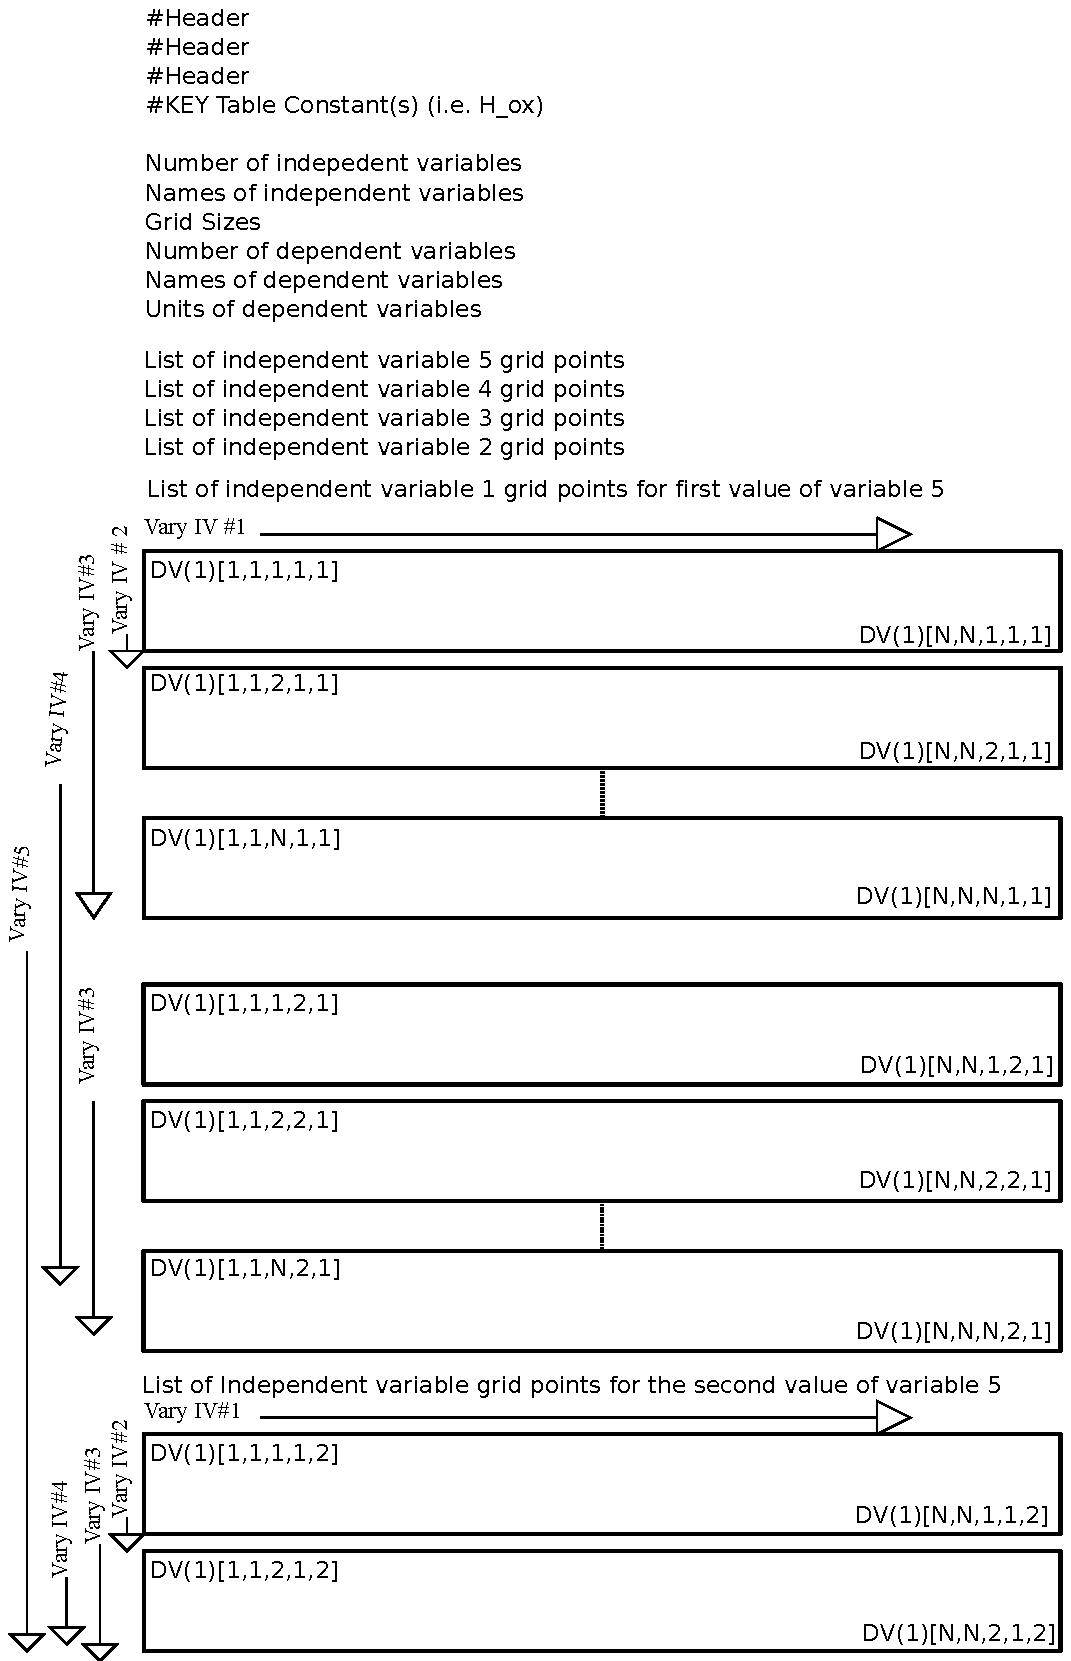
\includegraphics{TableDiagram.pdf}}
   \caption{Example 5D Table Layout}\label{fig:table_ex}
   \end{center}
\end{figure}

%\subsection{Extra Scalar Solvers}
%This section and all options will soon be replaced with Section \ref{Sec:AddTransEqn}. 

%\subsection{Additional Transport Equations}\label{Sec:AddTransEqn}


%\subsubsection{Turbulence}


%\subsubsection{Properties}


%\subsubsection{BoundaryConditions}


%\subsubsection{Physical Constants}


%\subsubsection{Solvers}


\subsection{Direct Quadrature Method of Moments}

The direct quadrature method of moments (DQMOM) is implemented in Arches, and various parameters, optional and required, are set in the input file. DQMOM involves transporting several transport equations, namely transport equations for the weights $w_{\alpha}$ and abscissas $ \left< \xi_{j} \right>_{\alpha}$, or, alternatively, the weights $w_{\alpha}$ and weighted abscissas $\varsigma_{j,\alpha}$.  Information about these transport equations must be specified in the DQMOM tags.

Three other things need to be specified, namely: a set of moments with which to generate a set of quadrature-approximated moment transport equations, which make up the linear system $\mathbf{Ax}=\mathbf{B}$; parameters related to the solver for the linear system $\mathbf{Ax} = \mathbf{B}$; and finally, physical models implemented to describe the evolution of the NDF in state-space. The input file has a DQMOM section denoted by the tag \verb=<DQMOM>=.

The basic structure is as follows:

% Add below, once completed:
%	<coalParticleCalculation>
%		...
%	</coalParticleCalculation>
\begin{Verbatim}[fontsize=\footnotesize]
<DQMOM>
	<LinearSolver>
		<!-- Linear solver options -->
		...
	</LinearSolver>
	
	<Models>
		<!-- the coal models used in DQMOM are specified here -->
		...
	</Models>
	
	<VelModel>
		<!-- information about the particle velocity model 
			is specified here -->
		...
	</VelModel>
	
	<Weights>
		<!-- weight transport equation information set here -->
		...
	</Weights>
	
	<Ic label="...">
		<!-- weighted abscissa (for each internal coordinate)
			transport equation information set here -->
		...
	</Ic>
	
	<Moment><m>[...]</m></Moment>
	...
	<Moment><m>[...]</m></Moment>
</DQMOM>
\end{Verbatim}

Three additional tags go between the \verb=<DQMOM>= tags.  These are:

\begin{enumerate}
%
\item {\bf Number of quadrature nodes}: \verb=<number_quad_nodes>= \\
{\bf Input type}: {\it Required, positive integer} \\
%{\bf Default}: {\it NA} \\
{\bf Description}: Denotes the number of quadrature nodes (also called environments) with which to represent the NDF. The NDF is represented by a set of delta function, and each quadrature node represents an additional delta function.
%
\item {\bf Adiabatic Gas, Non-Adiabatic Particles}: \verb=<adiabGas_nonadiabPart>= \\
{\bf Input type}: {\it Optional, boolean} \\
{\bf Default}: {\it false} \\
{\bf Description}: This parameter is used to indicate that the gas is adiabatic (in which case, it is {\it true}) and therefore heat loss should not be looked up from the table.  The default is to assume {\it false}, so that the heat loss will be used as a variable if it is so determined by the remainder of the input file.
% FIXME: This description needs some improvement
%
\item {\bf Save moments}: \verb=<save_moments>= \\
{\bf Input type}: {\it Optional, boolean} \\
{\bf Default}: {\it false} \\
{\bf Description}: This boolean determines whether or not the moments specified in the \verb=<Moments>= tags (see below) should be calculated in order to be saved out as variables.  If true, all moments specified in the \verb=<Moments>= tags will be calculated.  In order to actually save them, however, they must also be added to the \verb=<save>= labels.
%
\end{enumerate}



\subsubsection{Linear Solver, $<$LinearSolver$>$}
\begin{enumerate}
%
\item {\bf Tolerance}: \verb=<tolerance>= \\
{\bf Input type}: {\it Optional, positive double} \\
{\bf Default}: {\it } 1.0e-5 \\
{\bf Description}: Sets the linear solver tolerance for DQMOM.  For the linear system
%
\begin{equation}
\mathbf{Ax}=\mathbf{B},
\end{equation}
%
the residual vector $\mathbf{R}$ is defined as 
%
\begin{equation}
\mathbf{R} = \mathbf{Ax} - \mathbf{B}
\end{equation}
%
and the normalized residual vector $\mathbf{R^{\star}}$ is defined as 
%
\begin{equation}
\mathbf{R^{\star}} = \frac{ \mathbf{Ax} - \mathbf{B} }{ \mathbf{x} }.
\end{equation}
%
The tolerance set by this tag will enforce the following condition
%
\begin{equation}
\begin{cases}
\text{if} \Vert \mathbf{R^{\star}} \Vert \leq \text{tol} & \text{Use solution obtained from } \mathbf{x} = \mathbf{A^{-1}B} \\
\text{if} \Vert \mathbf{R^{\star}} \Vert > \text{tol} & \text{Throw out solution from } \mathbf{x} = \mathbf{A^{-1}B} \text{ and use } \mathbf{x = 0} \\
\end{cases}
\end{equation}
%
\item {\bf Type}: \verb=<type>= \\
{\bf Input type}: {\it Required, string} \\
{\bf Default}: {\it ``LU''} \\
{\bf Description}: The linear solver type; options are:
\begin{itemize}
\item ``Lapack-invert'' - uses a Lapack routine to invert $\mathbf{A}$, which is then multiplied by $\mathbf{B}$
\item ``Lapack-svd'' - uses a Lapack routine to calculate the singular value decomposition (SVD) of $\mathbf{A}$
\item ``LU'' - LU decomposition solver using the Crout's Method algorithm
\item ``Optimize'' - uses sets of optimal moments and optimal abscissas to get a well conditioned matrix
\end{itemize}
%
\item {\bf  Maximum allowable condition number for $\mathbf{A}$}: \verb=<maxConditionNumber>= \\
{\bf Input type}: {\it Optional, positive double} \\
{\bf Default}: {\it 1.0e+16} \\
{\bf Description }: If the condition number of $\mathbf{A}$ is greater than the maximum allowable condition number, the resulting solution vector is discarded and $\mathbf{x = 0}$ is used; this prevents large numerical errors from contaminating the solution.
%
\item {\bf Calculate condition number? (boolean)}: \verb=<calcConditionNumber>= \\
{\bf Input type}: {\it Optional, boolean} \\
{\bf Default}: {\it false} \\
{\bf Description }: If {\it true}, the condition number is calculated using singular value decomposition.  Note, this calculation is very expensive and should probably only be done when the ``Lapack-svd'' solver option is being used.  An error is thrown if this is true and the ``LU'' (Crout's Method) solver option is chosen.
%
\item {\bf Using the "Optimize" solver}: \verb=<Optimization>= \\
{\bf Description }: This section must be specified to use the "Optimize" solver. The section must contain specification of the optimal abscissas: \\
\verb=<Optimal_abscissas>= \\
{\bf Input type}: {\it Required, Vector} \\
{\bf Default}: {\it none} \\
{\bf Description }: The optimal abscissas should be specified as a vector (within brackets) and separated by comas. The set of moments chosen by the user should be consistent with the set of otpimal absissas. The number of optimal abscissas to specify is Nic*Nqn.  The user can use the matlab script located in $/src/StandAlone/inputs/ARCHES/matlab/find_optmoments.m$ to determine a set of optimal moments and absissas given a number of internal coordinates and quadrature nodes. After running the script, the set of optimal abscissas is stored in Xgood and the corresponding set of optimal moments is stored in Momentsgood. Note, the order of the abscissas and the moments matters and should not be changed. Also, the following options are irrelevent for the "Optimize" solver: tolerance, maxConditionNumber, calcConditionNumber. \\
%
\end{enumerate}



\subsubsection{Coal Models for DQMOM, $<$Models$>$}
See the \ref{subsec:models} section below for details about the \verb=<Models>= tag.



%\subsubsection{Iterative Coal Particle Calculation}



\subsubsection{Velocity Model}
%
This section sets parameters for the Balachandar velocity model.
%
\begin{enumerate}
%
\item {\bf Velocity model}: \verb=<VelModel>= \\
{\bf Attributes}: label, type \\
{\bf Description}: Attributes determine the label the velocity model is given, and the type of velocity model being used.  The label is an arbitrary string.  The type takes on these values:
\begin{itemize}
\item \verb=Balachandar= - Use the Balachandar particle velocity model
\item \verb=Dragforce= - Use a drag force law, and track particle velocity as an internal coordinate
\end{itemize}
%
\item {\bf Viscosity}: \verb=<kinematic_viscosity>= \\
{\bf Input type}: {\it Required, positive double} \\
{\bf Default}: {\it 1.0e-5} \\
{\bf Description}: The kinematic viscosity.
%
\item {\bf Length scale}: \verb=<L>= \\
{\bf Input type}: {\it Required, positive double} \\
{\bf Default}: {\it 1.0} \\
{\bf Description}: The integral scale of the simulation.
%
\item {\bf Density ratio}: \verb=<rho_ratio>= \\
{\bf Input type}: {\it Required, positive double} \\
{\bf Default}: {\it 1000} \\
{\bf Description}: The ratio of particle density to fluid density, $\dfrac{ \rho_{\text{particle}} }{ \rho_{\text{fluid}} }$.
%
\item {\bf Regime}: \verb=<regime>= \\
{\bf Input type}: {\it Required, integer (1 or 3)} \\
{\bf Default}: {\it 1} \\
{\bf Description}: The flow regime for the Balachandar particle velocity model.
%
\item {\bf Eta}: \verb=<eta>= \\
{\bf Input type}: {\it Required, positive double} \\
{\bf Default}: {\it 1.0e-5} \\
{\bf Description}: The Kolmogorov scale.
%
{\color[gray]{0.5}
\item {\bf High clip value (via upper limit multiplier)}: \verb=<upper_limit_multiplier>= \\
{\bf Input type}: {\it Optional, double} \\
{\bf Default}: {\it 2.0} \\
{\bf Description}: This factor is not actually used.  It is used to set a high clip value.  The way it stands in the code, this is, for some reason, multiplying the upper limit multiplier and the high clip value for the particle length - which doesn't make sense.
}
%
\item {\bf Low clip value}: \verb=<clip_low>= \\
{\bf Input type}: {\it Optional, double} \\
{\bf Default}: {\it 0.0} \\
{\bf Description}: Sets the low clip value for the particle velocity.
%
{\color[gray]{0.5}
\item {\bf Particle velocity boundary conditions}: \verb=<partvelBC_eq_gasvelBC>= \\
{\bf Input type}: {\it Optional, double} \\
{\bf Default}: {\it false} \\
{\bf Description}: If this value is true, the particle velocity boundary conditions are the same as the gas velocity boundary conditions.  \\
WARNING: This should NOT be turned on!  It will cause problems!
}
%
\item {\bf Minimum velocity ratio}: \verb=<min_vel_ratio>= \\
{\bf Input type}: {\it Optional, positive double} \\
{\bf Default}: {\it 0.1} \\
{\bf Description}: This keeps the particle velocity from becoming too different from the gas velocity.
%
\item {\bf Number of iterations}: \verb=<iter>= \\
{\bf Input type}: {\it Optional, positive integer} \\
{\bf Default}: {\it 15} \\
{\bf Description}: An iterative procedure is required to determine the particle velocity, since it appears in the Balachandar particle velocity model implicitly. This tag controls the maximum iterations that may be run.
%
\item {\bf Tolerance}: \verb=<tol>= \\
{\bf Input type}: {\it Optional, positive double} \\
{\bf Default}: {\it 1e-15} \\
{\bf Description}: This defines a maximum residual for the expression for the particle velocity appearing in the Balachandar particle velocity model; i.e., if $\left[ (LHS - RHS) \leq \text{tol} \right]$ then the iterative procedure finishes.
%
\end{enumerate}



\subsubsection{Weight Transport Equation Options, $<$Weights$>$}
%
\begin{enumerate}
%
\item {\bf Do Diffusion?}: \verb=<doDiff>= \\
{\bf Input type}: {\it Optional, boolean} \\
{\bf Default}: {\it false} \\
{\bf Description}: Boolean to determine whether transport equation's RHS will include a diffusion term. If true, it uses a turbulent Prandtl number to determine the diffusivity.  The turbulent Prandtl number can be set, but is 0.4 by default.  See \verb=<turbulentPrandtlNumber>= tag below.
%
\item {\bf Do Convection?}: \verb=<doConv>= \\
{\bf Input type}: {\it Optional, boolean} \\
{\bf Default}: {\it false} \\
{\bf Description}: Boolean to determine whether transport equation's RHS will include a convection term. Because the weights are DQMOM scalars, and the weight transport equations (originally) come from the NDF transport equation, the velocity used for the convection term is the particle velocity, conditioned on particle size.  This velocity comes from the DQMOM particle velocity model (see the \verb=<VelModel>= tag above).
%
\item {\bf Convection scheme}: \verb=<conv_scheme>= \\
{\bf Input type}: {\it Optional, string} \\
{\bf Default}: {\it upwind} \\
{\bf Description}: Tag to determine the convection scheme used. Valid options are:
\begin{itemize}
\item \verb=upwind= - use the upwind convection scheme
\item \verb=super_bee= - use the super-bee convection scheme
\end{itemize}
%
\item {\bf Turbulent Prandtl Number}: \verb=<turbulentPrandtlNumber>= \\
{\bf Input type}: {\it Optional, double} \\
{\bf Default}: {\it 0.4} \\
{\bf Description}: If diffusion is turned on, a turbulent Prandtl number is required to determine the diffusion coefficient.  The Prandtl number is defined as:
\begin{equation}
Pr = \dfrac{\nu}{D}
\end{equation}
where $\nu$ is the fluid viscosity, and $D$ is the scalar diffusivity.  This is equivalent to the turbulent Schmidt number.
%
\item {\bf Initialization function}: \verb=<initialization>= \\
{\bf Attributes}: type \\
{\bf Default}: none \\
{\bf Description}: There are several options for initialization functions. These are as follows:
%%
\begin{itemize}
\item {\it Constant value initialization}, \verb=constant= - Initializes the weights to be a constant throughout the domain; the constant value is the same for all weights of all environments. The block looks like:
\begin{Verbatim}
<initialization type="constant">
	<constant>...</constant>
</initialization>
\end{Verbatim}
where the \verb=<constant>= tags encapsulate a double.
%%
\item {\it Environment-specific constants}, \verb=env_constant= - Initializes the weights to be a constant throughout the domain; the constant value is different for the weights of each environment. The block looks like:
\begin{Verbatim}
<initialization type="env_constant" qn="..." value="...">
\end{Verbatim}
where ``qn'' is an integer specifying an environment (or quadrature node), and ``value'' is a double, and is the value to which the weight of that environment will be initialized.
%%
\item {\it Step-function initialization}, \verb=step= - Initializes the weights to be a step function. Several attributes of the step function must be specified; these include:
	\begin{itemize}
	\item \verb=<step_direction>= - Direction in which the step occurrs (x, y, z) (Required, no default)
	\item \verb=<step_value>= - The step goes from 0 to \verb=<step_value>= (double) (Required, no default)
	\item \verb=<step_start>= - Physical location at which step begins (double) (No default)
	\item \verb=<step_end>= - Physical location at which step ends (double) (No default)
	\item \verb=<step_cellstart>= - Cell location at which step begins (integer) (No default)
	\item \verb=<step_cellend>= - Cell location at which step ends (integer) (No default)
	\end{itemize}
The step function initialization block looks like:
\begin{Verbatim}
<initialization type="step">
	<step_direction> ... </step_direction>
	<step_value> ... </step_value>
	<step_start> ... </step_start>
	<step_end> ... </step_end>
</initialization>
\end{Verbatim}
or, alternatively, the start and end of the step could be specified using the cell locations, which would look like:
\begin{Verbatim}
<initialization type="step">
	<step_direction> ... </step_direction>
	<step_value> ... </step_value>
	<step_cellstart> ... </step_cellstart>
	<step_cellend> ... </step_cellend>
</initialization>
\end{Verbatim}
%%
\item {\it Environmental step-function initialization}, \verb=env_step= - Initializes the weights to step functions, with the value of the step function different for each environment. The attributes are the same as for the step-function initialization, except that the \verb=<step_value>= tag becomes a set of \verb=<env_step_value>= tags. These tags have the following attributes:
	\begin{itemize}
	\item \verb=qn= - the environment (or quadrature node) to which the \verb=<env_step_value>= tag applies
	\item \verb=value= - the value to which this environment's step function should be initialized
	\end{itemize}
so that the tags would look like:
\begin{Verbatim}
<initialization type="env_step">
	<step_direction> ... </step_direction>
	<step_start> ... </step_start>
	<step_end> ... </step_end>
	<env_step qn=" ... " value = " ... " >
	...
	<env_step qn=" ... "  value=" ... " >
</initialization>
\end{Verbatim}
%%
\end{itemize}
%
\item {\bf Scaling constant}: \verb=<scaling_const>= \\
{\bf Input type}: {\it Required, double} \\
{\bf Default}: {\it 1.0} \\
{\bf Description}: Value by which to scale the weights. The actual values of the weights are very high, as the weights represent numbers of particles (typically greater than 1e6). Because the values of the weights are going into the $\mathbf{A}$ matrix, large weight values can cause $\mathbf{A}$ to become very ill-conditioned. Scaling the values of the weights can help control condition numbers for $\mathbf{A}$.
%
\item {\bf Clipping}: \verb=<Clipping>= \\
{\bf Description}: Values of weights can attain non-physical values (e.g. negative numbers of particles, large and physically unrealistic numbers of particels, etc.). Clipping is implemented to prevent non-physical values.  The weights have three types of clipping:
	\begin{itemize}
	\item \verb=<low>= - Low clipping represents the lowest value the weights can attain (in most cases, 0)
	\item \verb=<small>= - As a result of the weight/weighted abscissa formulation of DQMOM, the abscissa values are not calculated by themselves; they are bound to the weights. Many models thus require dividing the weighted abscissas by the weights. When the weights become very small, this leads to physically unrealistic abscissa values. The small clipping sets a minimum value at which weights can divide weighted abscissas; when the weights are lower than this small clipping, the abscissas are set to 0.
	\item \verb=<high>= - High clipping represents an upper limit on values of weights.
	\end{itemize}
%
\end{enumerate}



\subsubsection{Weighted Abscissa Transport Equation Options, $<$Ic$>$}
%
Many of the options for the weighted abscissa transport equation options are the same as the weight transport equations. Only the differences are highlighted in this section.
%
\begin{enumerate}
%
\item {\bf Initialization}:
{\bf Description}: The initialization function options are more limited for weighted abscissas than for weights. If abscissas coincide, this creates singularities in $\mathbf{A}$. Thus, the constant and step function initialization functions must be environment-specific
%
\item {\bf Scaling constant}:
{\bf Description}: The scaling constant is for the abscissa, and not for the weighted abscissa. Because the weight is scaled, there are {\it two} scaling constants for each weighted abscissa: one scaling constant for the weights, the other for the abscissa.
%
\item {\bf Clipping}:
{\bf Description}: The clipping values are set for the abscissas, and not the weighted abscissas.  Additionally, there is no ``small'' clipping value, as there is no dividing by the abscissas.
%
\item {\bf Models}: \verb=<model>=
{\bf Attributes}: label \\
{\bf Description}: Attribute determines which model (identified by the label) should be associated with this internal coordinate. The label is an arbitrary string that must match a label for a model.
%
\end{enumerate}



\subsubsection{Moments, $<$Moment$>$}
%
An important part of DQMOM is selecting a set of moments that will be used to provide closure for the NDF. These moments are then used to construct the quadrature-approximated moment transport equations, which are written in the linear form $\mathbf{Ax} = \mathbf{B}$. The moments selected have a strong influence on the behavior of the matrix $\mathbf{A}$.
%
\begin{enumerate}
%
\item {\bf Moment}: \verb=<Moment>= \\
{\bf Input type}: {\it Required, multiple integers} \\
{\bf Default}: N/A \\
{\bf Description}: The moments are specified as sets of integer vectors. The \verb=<Moment>= block looks like:
\begin{Verbatim}
<Moment><m>[ ... , ... , ... ]</m></Moment>
...
<Moment><m>[ ... , ... , ... ]</m></Moment>
\end{Verbatim}
Note that the moment index vectors must be of size $N_{\xi}$, where $N_{\xi}$ is the number of internal coordinates, and there must be $\left( N_{\xi} + 1 \right) N$ total moments, where $N$ is the number of environments (or quadrature nodes).
%
\end{enumerate}



\subsubsection{Verification, $<$Verify\_Linear\_Solver$>$, $<$Verify\_AB\_Construction$>$}
%
Of major importance is the verification procedure for DQMOM. There are two important processes in the DQMOM code that must be verified: the construction of $\mathbf{Ax}=\mathbf{B}$, and the linear solver's solution to $\mathbf{Ax}={B}$. Both have verification mechanisms built in.
%
Verification is not something that can be ``turned on'' in the input file - it must be turned on using compiler directives.  The file Directives.h in the Arches component directory contains several directives related to verification, two of which are \verb=VERIFY_LINEAR_SOLVER= and \verb=VERIFY_AB_CONSTRUCTION=.
%
For verification, some additional information must be put into the input file. This information is specified for each verification procedure. Most of these tags point to files containing information which is used to construct $\mathbf{Ax}=\mathbf{B}$. These files are available in the Arches \verb=inputs/= directory.
%
\begin{enumerate}
%
\item {\bf Verification of Linear Solver}: \verb=<Verify_Linear_Solver>= \\
	\begin{itemize}
	\item \verb=<A>= - File containing A matrix
	\item \verb=<X>= - File containing X vector (verification solution)
	\item \verb=<B>= - File containing B vector
	\item \verb=<normR>= - File containing norm of the residual vector
	\item \verb=<norms>= - File containing several norms of vectors
	\item \verb=<dimension>= - The dimension of the linear system being solved
	\item \verb=<tolerance>= - Error tolerance
	\end{itemize}
%
\item {\bf Verification of A, B construction process}: \verb=<Verify_AB_Construction>= \\
	\begin{itemize}
	\item \verb=<A>= - File containing A matrix
	\item \verb=<B>= - File containing B vector
	\item \verb=<input>= - File containing various inputs (e.g. model terms)
	\item \verb=<moments>= - File containing moments
	\item \verb=<number_environments>= - Number of environments used to represent the NDF
	\item \verb=<number_internal_coordinates>= - Number of internal coordinates parameterizing the NDF
	\item \verb=<tolerance>= - Error tolerance
	\end{itemize}
%
\end{enumerate}



\subsection{Models}\label{subsec:models}
The $<$Models$>$ tags contain several tags that are not specific to models.  The outline of a typical $<$Models$>$ section looks like:

\begin{Verbatim}[fontsize=\footnotesize]
<Models>
	<model
	label = " ... "
	type  = " ... "   >

		<ICVars>

			<variable	
			label = " ... "
			role = " ... "  >

		</ICVars>

		<scalarVars>
		
			<variable	
			label = " ... "
			role   = " ... " >

		</scalarVars>

		<low_clip>  ... </low_clip>
		<high_clip> ... </high_clip>

	</model>
	
	...
	
</Models>
\end{Verbatim}

The sections have the following significance:

\begin{itemize}
\item \verb=<model>= - there is a \verb=<model>= tag block for each coal model
\item \verb=<ICVars>= - this tag block contains all of the internal coordinate variables that the model depends on (for example, if a kinetic model depends on temperature, and temperature is being tracked as an internal coordinate variable, the temperature would be included in this \verb=<ICVars>= block)
\item \verb=<scalarVars>= - this tag block contains all of the scalar variables that the model depends on
\item \verb=<low_clip>= - When values of the model are lower than \verb=<low_clip>=, the value is clipped to \verb=<low_clip>=
\item \verb=<high_clip>= - When values of the model are higher than \verb=<high_clip>=, the value is clipped to \verb=<high_clip>=
\end{itemize}

\begin{enumerate}

\item {\bf Model}: \verb=<model>= \\
{\bf Attributes}: label, type \\
{\bf Description}: Attributes determine the label the velocity model is given, and the type of velocity model being used.  The label is an arbitrary string.  The type takes on these values:
\begin{itemize}
\item \verb=KobayashiSarofimDevol= - Use the Kobayashi-Sarofim coal devolatilization model
\item \verb=ConstantModel= - Use a constant model
\item \verb=SimpleHeatTransfer= - Use a simple particle heat transfer model
\item \verb=XDrag, YDrag, ZDrag= - Use a standard drag model for the x-, y-, and z-velocity of the particle
\end{itemize}

\item {\bf Internal Coordinate Variable}: \verb=<ICVars> <variable> </ICVars>= \\
{\bf Attributes}: label, role \\
{\bf Description}: Attributes set the label of the internal coordinate variable, and the role that the internal coordinate variable plays in the model.  The label must match a label for one of the internal coordinate variables (see the ``label'' attribute of the \verb=<Ic>= tag, above).  The role must match one of the role names specified by the model, in the model code.  These include:
\begin{itemize}

\item KobayashiSarofimDevol
	\begin{itemize}
	\item \verb=raw_coal_mass=
	\item \verb=particle_temperature=
	\end{itemize}

\item SimpleHeatTransfer
	\begin{itemize}
	\item \verb=particle_length=
	\item \verb=raw_coal_mass=
	\item \verb=particle_temperature=
	\end{itemize}

\item XDrag / YDrag / ZDrag
	\begin{itemize}
	\item \verb=particle_length=
	\item \verb=particle_xvel / particle_yvel / particle_zvel=
	\end{itemize}

\end{itemize}

\item {\bf Scalar Variable}: \verb=<scalarVars> <variable> </scalarVars>= \\
{\bf Attributes}: label, role \\
{\bf Description}: As with the above \verb=<variable>= tag, this tag specifies information about scalar variables a model may depend on. The label attribute indicates the label of the scalar variable, and the role specifies the role that scalar variable will play in the model. The label attribute must match a label for one of the scalar variables. The role must match one of the role names specified by the model, in the model code.  Currently, scalar variables do not play a role in any models currently implemented.

\end{enumerate}


\subsection{Digital Filter Generator}
In order to utilize the digital filter turbulent inlet condition  in \ref{subsubsec:TurbInlet}, the executable \verb=DigitalFilterGenerator= is the best way to generate the table needed.  This executable lies in the \verb=StandAlone= folder.  Its usage is simply 

\begin{verbatim}
./DigitalFilterGenerator input_file output_table_file
\end{verbatim}

If not output table file is specified this writes out to \verb=DFGInlet=.  The input file is a small text file with the grid size and geometries specified on individual lines.  Currently it must be specified in a specific order.

\begin{enumerate}
\item Grid resolution \verb=<int> <int> <int>=
\item Lower grid points \verb=<double> <double> <double>=
\item Upper grid points \verb=<double> <double> <double>=
\item Inlet face \verb=<string>= (x+, x-, y-, y+, z-, z+)
\item Inlet geometry shape \verb=<string>= (box/circle/ellipse/annulus)
\item Geometry parameters \verb=<double>= (varies on geometry, same order as BCGeom objects )
\item Number of realizations in file \verb=<int>=
\item Lengthscales \verb=<double> <double> <double>=
\item Accuracy of filter (min 2) \verb=<double>=
\item Average velocity vector \verb=<double> <double> <double>=
\item Average Reynold's stress tensor (lower diagonal) \verb=<double> <double> <double>= \\
\verb=<double> <double> <double>= $R_{11},\; R_{21},\; R_{22},\; R_{31},\; R_{32},\; R_{33} $
\item Use spatial variations \verb=<string>= (y, yes, n, no)
\item Variation direction \verb=<string>= (x, y, z, none) used if a planar geometric relation is needed
\item Velocity variation type \verb=<string>= (tanh, power, laminar, none)
\item Stress variation type \verb=<string>= (channel, jet, none)
\item Lengthscale variation type \verb=<string>= (channel, jet, none)
\end{enumerate}

An example input file for the digital filter is located in \\ \verb=StandAlone/inputs/ARCHES/DigitalFilter/ChannelInletGenerator.txt=.  It is recommended to gzip the file that is created to save space.


 
% ====================================================
% ===================== Examples ======================
% ====================================================



\newpage
\section{Examples}

The following ARCHES examples illustrate the diverse set of problems that can be solved using the ARCHES component of Uintah code.  The first two examples exemplify techniques used to verify various ARCHES algorithms that were implemented in the code.  The following three [or more] examples illustrate the kinds of problems that ARCHES can solve.  The input files used here can be used as templates to build similar input files for similar problems. 
Due to the complexity of ARCHES simulations, exact solutions (with the exception of MMS) do not exist.  Hence the emphasis on model validation, or the comparison of simulation with experimental results.  Model validation provides a framework that allows the simulation scientist to be confident in his or her results in the absence of analytical solutions.  All modeling should be accompanied by some form of validation analysis.


\subsection*{\center Almgren MMS}
\addcontentsline{toc}{subsection}{Almgren MMS}
\subsubsection*{\underline{Problem Description}}

Methods of Manufactured Solutions (MMS) are verification tools that are used with computer codes such as ARCHES that seek to solve the Navier-Stokes Equations.  They are extremely useful for finding programming errors and ensuring expected behavior of the computer code.   The Almgren MMS is especially easy to implement because of the absence of source terms that must be added to the transport equations.
ARCHES uses a second-order spatial discretization scheme and a first-order scheme in the temporal direction.  Therefore, if the Almgren MMS problem is run in Arches at different mesh resolutions and the normalized error plotted on a semilog plot, the slope of the line should be 2.  To facilitate this exercise, a shell script has been written to perform this analysis.

\subsubsection*{\underline{Simulation Specifics}}
\begin{description} 
\footnotesize
\item [Component used:] \hfill ARCHES
\item [Input file name:] \hfill \TT{almgrenMMS.ups}\\
\item [Command used to run input file:]\hfill \\

% Write .sh script to run almgrenMMS.ups 4 times at different resolutions [32,32,8], [24,24,8]. [12,12,8], and [8,8,8] and then extract L2norms to a .dat file that can easily be plotted in Excel or Matlab.
\TT{./runAlmgren.sh }

If you examine the shell script you will see the following line of code:
\TT{mpirun -np 1 sus  inputs/UintahRelease/ARCHES/almgrenMMS.ups}
This is call to run the ARCHES via sus.

\item [Simulation Domain:]\hfill    1.0 x 1.0 x 3.0 m
\item [Cell Spacing:]\hfill \\ 
0.3125 x 0.3125 x 0.275 m

\item [Example Runtimes:] \hfill \\
113.2 seconds (1 processor, 2.4 GHz Intel Core 2)

\item [Physical time simulated:] \hfill \\
  1.0 sec.
\end{description}

%%%%%%%%%%%%%%%%%%%%%%%%%%%%%%%%%%%%
% Figure showing plot of error as a function of spatial discretization
 %%%%%%%%%%%%%%%%%%%%%%%%%%%%%%%%%%%%
 
 %--------------------------------------------------------------
 \newpage
\subsection*{\center Periodic Box Problem}
\addcontentsline{toc}{subsection}{Periodic Box Problem}
\subsubsection*{\underline{Problem Description}}

The Periodic Box Problem indicates how well ARCHES is modeling the
kinetic energy contained in the turbulence modeled on the grid and at
a sub-grid level.  The LES algorithm transfers kinetic energy from
cell to cell in the ARCHES structured grid. Turbulence models such as
"compdynamicprocedure," "dynamicprocedure," and "smagorinsky" are used
to model kinetic energy at the sub-grid level.  Ideally, there would
be a seamless transition between the resolved turbulence and sub-grid
models at the Nyquist limit.  {\bf SHOW SAMPLE PLOT}  Experience has shown that this is not normally the case.   By plotting the kinetic energy as a function of the wave number, it is possible to determine how well the kinetic energy dissipation is being modeled by the code.  The Periodic Box problem is initialized with a kinetic energy (turbulence) profile from Direct Numerical Simulation (DNS).  As the simulation proceeds that energy is dissipated.  
 % COMPLETE ME

\subsubsection*{\underline{Simulation Specifics}}
\begin{description} 
\footnotesize
\item [Component used:] \hfill ARCHES
\item [Input file name:] \hfill \TT{periodic.ups}\\
 
\item [Command used to run input file:]\hfill \\
This simulation, like many ARCHES simulations, requires another file, in addition to the input file called by sus.  That file is the initial condition called upon in periodic.ups by %<set\_initial\_condition inputfile\="iso\_ini\_32.dat"/>

\TT{mpirun -np 1 sus  inputs/UintahRelease/ARCHES/periodic.ups  }  % I am using the periodic.ups file found in the tree

\item [Simulation Domain:]\hfill    0.565 x 0.565 x 0.565 m
\item [Cell Spacing:]\hfill \\ 
0.0177 x 0.0177 x 0.0177 m  %[32]^3

\item [Example Runtimes:] \hfill \\
2 minutes   (1 processor, 2.4 GHz Intel Core 2 )

\item [Physical time simulated:] \hfill \\
0.1 sec.  % Is this time long enough???
\end{description}

%%%%%%%%%%%%%%%%%%%%%%%%%%%%%%%%%%%%
% Figure showing plot of kinetic energy as a function of the wave number
%
% +  Discussion
%
 %%%%%%%%%%%%%%%%%%%%%%%%%%%%%%%%%%%%

 %--------------------------------------------------------------
\newpage
\subsection*{\center Helium Plume}
\addcontentsline{toc}{subsection}{Helium Plume}
\subsubsection*{\underline{Problem Description}}
Helium plumes are classical experiments that allow for the easy
capture of turbulent mixing data that can be used to validate the
turbulent mixing models used in LES algorithms such as Arches.  The
non-reacting nature of the plume makes it easy to capture experimental
data without damaging expensive equipment.  Reacting flows require
special mixing tables that contain temperature, pressure and
composition as a function of the transported scalars in Arches.  The
coldFlowMixingModel is used to determine the mixing of {\bf isothermal?} streams.  After the mixing model is specific in the .ups file, the temperature and densities of the two mixing streams are specified.

\subsubsection*{\underline{Simulation Specifics}}
\begin{description} 
\footnotesize
\item [Component used:] \hfill ARCHES
\item [Input file name:] \hfill \TT{helium\_1m.ups}\\
 
\item [Command used to run input file:]\hfill \\
\TT{mpirun -np 8 sus  inputs/UintahRelease/ARCHES/helium\_1m.ups  }

\item [Simulation Domain:]\hfill    3.0 x 3.0 x 3.0 m
\item [Cell Spacing:]\hfill \\ 
0.06 x 0.06 x 0.0.6 m

\item [Example Runtimes:] \hfill \\
 54 minutes   (8 processors, 2.8 GHz Xeon)

\item [Physical time simulated:] \hfill \\
  5.0 sec.
\end{description}

\subsubsection*{\underline{Results}}

%%%%%%%%%%%%%%%%%%%%%%%%%%%%%%%%%%%%
% Image from [300]^3 simulation
%
% Plot from Diem's work with the Sandia Helium Plume dataset
%%%%%%%%%%%%%%%%%%%%%%%%%%%%%%%%%%%%

 %--------------------------------------------------------------
\newpage
\subsection*{\center Methane Plume}
\addcontentsline{toc}{subsection}{Methane Plume}
\subsubsection*{\underline{Problem Description}}
This methane plume is geometrically identical to the Helium Plume problem.  The difference is the addition of chemistry.  Instead of unreacting, isothermal fluids mixing, a fuel is reacting to combustion products inside of the computational domain.  This chemistry is captured via a mixing table.  The input file is pointed to the mixing table which contains state variables and species mass fractions as a function of mixture fraction, heat loss, and mixture fraction variance.   

\subsubsection*{\underline{Simulation Specifics}}
\begin{description} 
\footnotesize
\item [Component used:] \hfill ARCHES
\item [Input file name:] \hfill \TT{helium\_1m.ups}\\
Note that the input file is pointed to the mixing table (inputs/UintahRelease/ARCHES/CH4\_equil\_clipped.mxn.gz)
 
\item [Command used to run input file:]\hfill \\
\TT{mpirun -np 8 sus  inputs/UintahRelease/ARCHES/helium\_1m.ups  }

\item [Simulation Domain:]\hfill    3.0 x 3.0 x 3.0 m
\item [Cell Spacing:]\hfill \\ 
0.06 x 0.06 x 0.0.6 m

\item [Example Runtimes:] \hfill \\
 2 hours 10 minutes   (8 processors, 2.8 GHz Xeon)

\item [Physical time simulated:] \hfill \\
  5.0 sec.
\end{description}

\subsubsection*{\underline{Results}}
% Discussion of ...?

%%%%%%%%%%%%%%%%%%%%%%%%%%%%%%%%%%%%%
% Nifty manta image with realistic looking flame
% Specify characteristics of simulation
%%%%%%%%%%%%%%%%%%%%%%%%%%%%%%%%%%%%%

 %--------------------------------------------------------------
\newpage
\subsection*{\center Fast Cookoff}
\addcontentsline{toc}{subsection}{Fast Cookoff}
\subsubsection*{\underline{Problem Description}}
The Fast Cookoff test is a procedure used for hazard classification of energetic materials.  The object is immersed over a jet fuel pool fire and the reaction, if any, is observed.  Current protocol requires that the full size article must be subjected to this test, making such procedures prohibitively expensive and unfeasible for articles such as solid rocket motors.  An alternative procedure has been proposed, combining sub-scale experiments with computer simulation.  Through validation and uncertainty quantification procedures, the computer simulation tool (ARCHES) can be used as a surrogate for full-scale experimental testing.  This Fast Cookoff problem includes a reacting flow as well as an MPMARCHES object.  After performing the simulation, the incident heat flux to the cylinder can be extracted.  

\subsubsection*{\underline{Simulation Specifics}}
\begin{description} 
\footnotesize
\item [Component used:] \hfill MPMARCHES

\item [Input file name:] \hfill \TT{fastcookoff.ups}\\

\item [Command used to run input file:]\hfill \\
Note that the input file is pointed to the mixing table (inputs/UintahRelease/ARCHES/sandia\_jp8\_flmlt\_cg.mxn)

\TT{mpirun -np 64 sus  inputs/UintahRelease/ARCHES/fastcookoff.ups  }
To extract the incident heat flux to the cylinder, use the faceextract and timeextract utilities.  <How to do this>

\item [Simulation Domain:]\hfill    24.0 x 24.0 x 24.0 m
\item [Cell Spacing:]\hfill \\ 
0.24 x 0.24 x 0.24 m

\item [Example Runtimes:] \hfill \\
7 hours 27 minutes   (64 processors, 2.8 GHz Xeon)  % UDA at /scratch/uintah/hinckley/ARCHES_examples

\item [Physical time simulated:] \hfill \\
  10.0 sec.
\end{description}

\subsubsection*{\underline{Results}}


\section{References}
\bibliographystyle{plain}
\bibliography{arches}
